% This is the Reed College LaTeX thesis template. Most of the work
% for the document class was done by Sam Noble (SN), as well as this
% template. Later comments etc. by Ben Salzberg (BTS). Additional
% restructuring and APA support by Jess Youngberg (JY).
% Your comments and suggestions are more than welcome; please email
% them to cus@reed.edu
%
% See http://web.reed.edu/cis/help/latex.html for help. There are a
% great bunch of help pages there, with notes on
% getting started, bibtex, etc. Go there and read it if you're not
% already familiar with LaTeX.
%
% Any line that starts with a percent symbol is a comment.
% They won't show up in the document, and are useful for notes
% to yourself and explaining commands.
% Commenting also removes a line from the document;
% very handy for troubleshooting problems. -BTS

% As far as I know, this follows the requirements laid out in
% the 2002-2003 Senior Handbook. Ask a librarian to check the
% document before binding. -SN

%%
%% Preamble
%%
% \documentclass{<something>} must begin each LaTeX document
\documentclass[12pt,twoside]{reedthesis}
% Packages are extensions to the basic LaTeX functions. Whatever you
% want to typeset, there is probably a package out there for it.
% Chemistry (chemtex), screenplays, you name it.
% Check out CTAN to see: http://www.ctan.org/
%%
\usepackage{graphicx,latexsym}
\usepackage{amsmath}
\usepackage{amssymb,amsthm}
\usepackage{longtable,booktabs,setspace}
\usepackage{chemarr} %% Useful for one reaction arrow, useless if you're not a chem major
\usepackage[hyphens]{url}
% Added by CII
\usepackage{hyperref}
\usepackage{lmodern}
\usepackage{float}
\floatplacement{figure}{H}
% End of CII addition
\usepackage{rotating}

% Next line commented out by CII
%%% \usepackage{natbib}
% Comment out the natbib line above and uncomment the following two lines to use the new
% biblatex-chicago style, for Chicago A. Also make some changes at the end where the
% bibliography is included.
%\usepackage{biblatex-chicago}
%\bibliography{thesis}


% Added by CII (Thanks, Hadley!)
% Use ref for internal links
\renewcommand{\hyperref}[2][???]{\autoref{#1}}
\def\chapterautorefname{Chapter}
\def\sectionautorefname{Section}
\def\subsectionautorefname{Subsection}
% End of CII addition

% Added by CII
\usepackage{caption}
\captionsetup{width=5in}
% End of CII addition

% \usepackage{times} % other fonts are available like times, bookman, charter, palatino

% Syntax highlighting #22

% To pass between YAML and LaTeX the dollar signs are added by CII
\title{Proto-Solutrean lithic technology of Western Iberia: sites of Vale Boi and Lapa do Picareiro}
\author{Joana Belmiro}
% The month and year that you submit your FINAL draft TO THE LIBRARY (May or December)
\date{May 2020}
\division{Faculdade de Ciências Humanas e Sociais}
\advisor{João Cascalheira}
\institution{Universidade do Algarve}
\degree{Mestrado em Arqueologia}
%If you have two advisors for some reason, you can use the following
% Uncommented out by CII
% End of CII addition

%%% Remember to use the correct department!
\department{Arqueologia}
% if you're writing a thesis in an interdisciplinary major,
% uncomment the line below and change the text as appropriate.
% check the Senior Handbook if unsure.
%\thedivisionof{The Established Interdisciplinary Committee for}
% if you want the approval page to say "Approved for the Committee",
% uncomment the next line
%\approvedforthe{Committee}

% Added by CII
%%% Copied from knitr
%% maxwidth is the original width if it's less than linewidth
%% otherwise use linewidth (to make sure the graphics do not exceed the margin)
\makeatletter
\def\maxwidth{ %
  \ifdim\Gin@nat@width>\linewidth
    \linewidth
  \else
    \Gin@nat@width
  \fi
}
\makeatother

\renewcommand{\contentsname}{Table of Contents}
% End of CII addition

\setlength{\parskip}{0pt}

% Added by CII

\providecommand{\tightlist}{%
  \setlength{\itemsep}{0pt}\setlength{\parskip}{0pt}}

\Acknowledgements{

}

\Dedication{

}

\Preface{

}

\Abstract{
The present thesis aims to answer the following question: what impact did the Heinrich 2 event have on the technological organization of human communities, on the onset of the last glacial maximum, in south western Iberia? This question follows the understanding that climatic events such as the HE2 seem to correlate to cultural changes, although the existing models do not consider the Proto-Solutrean technocomplex as an individual phase for the Gravettian-Solutrean transition, thus leaving a gap in the current knowledge of the Upper Paleolithic.

\par

To approach this problematic we analysed the lithic assemblages from Vale Boi (south Portugal) and Lapa do Picareiro (central Portugal) to understand the technological patterns and territory exploitation during the Proto-Solutrean, with the following goals: 1) understand and explain specific site technological and raw material use patterns; 2) establish parallels between the two sites; 3) compare these results with those obtained for other Proto-Solutrean sites, mostly from the Portuguese Estremadura.

The analysis followed a technologic and morphologic attribute approach, with the statistical treatment of data through descriptive and multivariate analysis, the latter through the use of a technological domain approach to reduce assemblage variability.

Results --

Keywords: Upper Paleolithic; Technological patterns; Raw material exploitation.
}

\Resumo{
O objetivo desta tese é responder à seguinte pergunta: que impacto teve o evento climático Heinrich 2 (HE 2) na organização tecnológica das comunidades de caçadores-recolectores no início do último máximo glacial (LGM), no sudoeste peninsular?

\par

Esta questão está intimamente ligada ao entendimento de certos eventos climáticos abruptos, tais como os eventos de Heinrich ou os Estados Glaciares, com a substituição de culturas ao longo do Paleolítico Superior. Um destes momentos de substituição correlaciona a passagem do Gravetense para o Solutrense com o evento HE 2 e com o Estádio Glacial 3, possivelmente sobreposta pelo LGM. Neste paradigma, as mudanças climáticas desencadeiam mudanças sociais, através do colapso de tradições que depois são reorganizadas, de forma a corresponder às novas condições ambientais e paisagísticas. No entanto, nos modelos existentes, o Proto-Solutrense não surge como um tecnocomplexo individualizado, existindo assim uma lacuna no entendimento atual do processo de transição entre os dois horizontes culturais supramencionados.

O Proto-Solutrense, representado sobretudo na Estremadura Portuguesa, é entendido como um tecnocomplexo de transição, ocorrendo entre os 26 000 cal BP e 25 400 cal BP, e caracterizado por mudanças na tecnologia e preferência de matérias-primas, existindo dois modelos para a sua evolução: modelo em duas etapas; e modelo em três etapas.

O modelo em duas etapas considera a existência do Gravetense Final e Proto-Solutrense, caracterizado pelo uso intensivo de quartzo e estratégias de produção para obtenção de lamelas em núcleos carenados e obtenção de suportes convergentes para pontas de Vale Comprido, sendo, no entanto, caracterizado por uma alta variabilidade interna. O modelo em três etapas consiste na evolução do Gravetense Final para uma etapa intermédia (no modelo das duas etapas considerada uma fácies funcional do Proto-Solutrense), caracterizada pelo uso intensivo do quartzo, estratégias de redução para obtenção de lamelas em núcleos carenados, seguida de uma fase Proto-Solutrense caracterizada pela diminuição do uso do quartzo e estratégias de redução para obtenção de suportes convergentes para pontas de Vale Comprido.
O conhecimento atual do Proto-Solutrense apresenta-se truncado, no entanto, pela antiguidade de algumas escavações e a sua restrição geográfica à Estremadura Portuguesa.

De forma a responder à questão supramencionada, assim como contribuir para o conhecimento do Proto-Solutrense no sudoeste Peninsular, foram analisados os conjuntos líticos de Vale Boi (sul de Portugal) e Lapa do Picareiro (Portugal central), ambos escavados nos últimos 20 anos com recurso a estações totais. Esta análise teve a finalidade de entender os padrões tecnológicos e de exploração do território durante o Proto-Solutrense, através dos seguintes objetivos: 1) entender e explicar os padrões tecnológicos e de preferência de matérias-primas intra-sítio; 2) estabelecer paralelos entre os dois sítios; 3) comparar estes resultados com os obtidos em outros sítios com conjuntos Proto-Solutrenses, sobretudo da Estremadura.

A análise seguiu uma abordagem de atributos tecnológicos e morfológicos, seguida de uma fase de tratamento estatístico através de duas metodologias: estatística descritiva e multivariada, ambas efetuadas em ambiente R. A análise multivariada segue a metodologia já descrita noutros trabalhos (Tostevin 2012; Scerri et al.~2014), e que passa pelo agrupamento de vários atributos em domínios tecnológicos, cada qual representando uma escolha do talhador(a) em alturas chave do talhe, de forma a reduzir a variabilidade interna dos conjuntos.

Palavras-chave: Paleolítico Superior; Padrões tecnológicos; Exploração de matérias-primas.
}

	\usepackage[T1]{fontenc}
\usepackage[utf8]{inputenc}
	\usepackage{booktabs}
\usepackage{longtable}
\usepackage{array}
\usepackage{multirow}
\usepackage{wrapfig}
\usepackage{float}
\usepackage{colortbl}
\usepackage{pdflscape}
\usepackage{tabu}
\usepackage{threeparttable}
\usepackage{threeparttablex}
\usepackage[normalem]{ulem}
\usepackage{makecell}
\usepackage{xcolor}
% End of CII addition
%%
%% End Preamble
%%
%
\begin{document}

% Everything below added by CII
  \maketitle

\frontmatter % this stuff will be roman-numbered
%\pagestyle{empty} % this removes page numbers from the frontmatter


  \begin{abstract}
    The present thesis aims to answer the following question: what impact did the Heinrich 2 event have on the technological organization of human communities, on the onset of the last glacial maximum, in south western Iberia? This question follows the understanding that climatic events such as the HE2 seem to correlate to cultural changes, although the existing models do not consider the Proto-Solutrean technocomplex as an individual phase for the Gravettian-Solutrean transition, thus leaving a gap in the current knowledge of the Upper Paleolithic.
    
    \par
    
    To approach this problematic we analysed the lithic assemblages from Vale Boi (south Portugal) and Lapa do Picareiro (central Portugal) to understand the technological patterns and territory exploitation during the Proto-Solutrean, with the following goals: 1) understand and explain specific site technological and raw material use patterns; 2) establish parallels between the two sites; 3) compare these results with those obtained for other Proto-Solutrean sites, mostly from the Portuguese Estremadura.
    
    The analysis followed a technologic and morphologic attribute approach, with the statistical treatment of data through descriptive and multivariate analysis, the latter through the use of a technological domain approach to reduce assemblage variability.
    
    Results --
    
    Keywords: Upper Paleolithic; Technological patterns; Raw material exploitation.
  \end{abstract}
  \begin{resumo}
    O objetivo desta tese é responder à seguinte pergunta: que impacto teve o evento climático Heinrich 2 (HE 2) na organização tecnológica das comunidades de caçadores-recolectores no início do último máximo glacial (LGM), no sudoeste peninsular?
    
    \par
    
    Esta questão está intimamente ligada ao entendimento de certos eventos climáticos abruptos, tais como os eventos de Heinrich ou os Estados Glaciares, com a substituição de culturas ao longo do Paleolítico Superior. Um destes momentos de substituição correlaciona a passagem do Gravetense para o Solutrense com o evento HE 2 e com o Estádio Glacial 3, possivelmente sobreposta pelo LGM. Neste paradigma, as mudanças climáticas desencadeiam mudanças sociais, através do colapso de tradições que depois são reorganizadas, de forma a corresponder às novas condições ambientais e paisagísticas. No entanto, nos modelos existentes, o Proto-Solutrense não surge como um tecnocomplexo individualizado, existindo assim uma lacuna no entendimento atual do processo de transição entre os dois horizontes culturais supramencionados.
    
    O Proto-Solutrense, representado sobretudo na Estremadura Portuguesa, é entendido como um tecnocomplexo de transição, ocorrendo entre os 26 000 cal BP e 25 400 cal BP, e caracterizado por mudanças na tecnologia e preferência de matérias-primas, existindo dois modelos para a sua evolução: modelo em duas etapas; e modelo em três etapas.
    
    O modelo em duas etapas considera a existência do Gravetense Final e Proto-Solutrense, caracterizado pelo uso intensivo de quartzo e estratégias de produção para obtenção de lamelas em núcleos carenados e obtenção de suportes convergentes para pontas de Vale Comprido, sendo, no entanto, caracterizado por uma alta variabilidade interna. O modelo em três etapas consiste na evolução do Gravetense Final para uma etapa intermédia (no modelo das duas etapas considerada uma fácies funcional do Proto-Solutrense), caracterizada pelo uso intensivo do quartzo, estratégias de redução para obtenção de lamelas em núcleos carenados, seguida de uma fase Proto-Solutrense caracterizada pela diminuição do uso do quartzo e estratégias de redução para obtenção de suportes convergentes para pontas de Vale Comprido.
    O conhecimento atual do Proto-Solutrense apresenta-se truncado, no entanto, pela antiguidade de algumas escavações e a sua restrição geográfica à Estremadura Portuguesa.
    
    De forma a responder à questão supramencionada, assim como contribuir para o conhecimento do Proto-Solutrense no sudoeste Peninsular, foram analisados os conjuntos líticos de Vale Boi (sul de Portugal) e Lapa do Picareiro (Portugal central), ambos escavados nos últimos 20 anos com recurso a estações totais. Esta análise teve a finalidade de entender os padrões tecnológicos e de exploração do território durante o Proto-Solutrense, através dos seguintes objetivos: 1) entender e explicar os padrões tecnológicos e de preferência de matérias-primas intra-sítio; 2) estabelecer paralelos entre os dois sítios; 3) comparar estes resultados com os obtidos em outros sítios com conjuntos Proto-Solutrenses, sobretudo da Estremadura.
    
    A análise seguiu uma abordagem de atributos tecnológicos e morfológicos, seguida de uma fase de tratamento estatístico através de duas metodologias: estatística descritiva e multivariada, ambas efetuadas em ambiente R. A análise multivariada segue a metodologia já descrita noutros trabalhos (Tostevin 2012; Scerri et al.~2014), e que passa pelo agrupamento de vários atributos em domínios tecnológicos, cada qual representando uma escolha do talhador(a) em alturas chave do talhe, de forma a reduzir a variabilidade interna dos conjuntos.
    
    Palavras-chave: Paleolítico Superior; Padrões tecnológicos; Exploração de matérias-primas.
  \end{resumo}
  \hypersetup{linkcolor=black}
  \setcounter{tocdepth}{2}
  \tableofcontents

  \listoftables

  \listoffigures


\mainmatter % here the regular arabic numbering starts
\pagestyle{fancyplain} % turns page numbering back on

\hypertarget{if-you-have-more-two-advisors-un-silence-line-7}{%
\chapter{If you have more two advisors, un-silence line 7}\label{if-you-have-more-two-advisors-un-silence-line-7}}

Placeholder

\hypertarget{introduction}{%
\chapter{Introduction}\label{introduction}}

The replacement of the Gravettian culture by the Solutrean, impacted by the adverse climatic conditions onset by the Heinrich Event 2 and its development through the last glacial maximum, continues to be an essential topic for understanding the Upper Paleolithic and Human adaptations. The Proto-Solutrean is, in this topic, an essential piece to understand how hunter-gatherer communities adapted, reinvented and destroyed behaviours that eventually allowed the development of the Solutrean. However, the existing knowledge on this technocomplex is still geographically constricted and lacking good chronological markers (Cascalheira and Bicho 2013), which hampers the understanding of the Proto-Solutrean itself and its role in the transition between the Gravettian and Solutrean technocomplexes.

By understanding the need of a better understanding of the Proto-Solutrean and how adverse climate impacted these communities, this thesis aims to answer the following question: what impact did the Heinrich 2 event have on the technological organization of human communities, on the onset of the last glacial maximum, in south western Iberia?

To answer this question, the present thesis has a number of goals, each connected to a problematic regarding the topic at hand, which will be met with resource to the lithic proto-solutrean assemblages of two sites, Vale Boi (south of Portugal) and Lapa do Picareiro (central Portugal).

To understand technological organization, our goal is to characterize and understand technological patterns, reduction sequences and assemblage variability in Proto-Solutrean occupations for both sites, as well as comprehend raw material use and preference patterns. The results will then be compared with the existing data from other Proto-Solutrean assemblages, mostly from the Estremadura Portuguesa area.

To better comprehend the transition from the Gravettian into the Solutrean, and how climate might have impacted this transition, we aim to test the existing Proto-Solutrean transitional models, the Two-phase and Three-phase, and understand how the two studied sites fit within the models, and whether there exists geographic variability. To do so, two question need to be answered: 1) if the proto-solutrean layers in Vale Boi show a Terminal Gravettian horizon; 2) if the two identified proto-solutrean phases in Lapa do Picareiro (Terminal Gravettian and Proto-Solutrean) show chronological significance.

Through the accomplishment of these goals, we hope to contribute to the understanding of the Proto-Solutrean in western Iberia, but also to the topic of the Gravettian culture replacement and subsequentially, the appearance of the Solutrean, through new data resulting from recent excavations and a wider geographic range (extending the knowledge of this transition to the south of Portugal).

The present thesis is organized in 9 chapters. Chapter 2, which follows the present introduction, will offer some contextualization on the human adaptations which characterize the start of the last glacial maximum, starting with a brief review of paleoclimate during the Upper Paleolithic in western Iberia, the several climate events and their relationship with cultural systems, and finishing with a brief overview of the Proto-Solutrean, its origins, chronology, technological characteristics and evolution models.

On chapter 3 we will introduce the archaeological site of Vale Boi, with a brief description of its localization and geological context, followed by an overview of excavation works, excavation methodology, human occupation layers through the several areas, and stratigraphy of the Terrace area, with particular focus on layer 4E and 5, the Proto-Solutrean occupation layers.

Chapter 4 follows the same organization as the previous chapter, this time focusing on the introduction of the archaeological site of Lapa do Picareiro, on the final part describing instead layers U and T which correspond to the Terminal Gravettian and Proto-Solutrean occupations.

Chapter 5 is dedicated to the description of the methodology employed in both the lithic assemblage analysis and data analysis.

Chapter 6 and 7 will follow the same structure, to present the results obtained in the analysis of the assemblage from Vale Boi and Lapa do Picareiro respectively. As such, the chapters are divided between assemblage description, raw materials and technology, this latter subsection presenting results from the descriptive and multivariate analysis.

Chapter 8 will consist on the discussion of both the results shown in the previous chapters, whenever possible connecting and comparing them, and extending this comparison to other results from Proto-Solutrean assemblages, mostly from the Portuguese Estremadura.

Chapter 9 offers some conclusions, systematizing the analysis interpretations and discussion.

\hypertarget{human-adaptations-at-the-start-of-the-last-glacial-maximum}{%
\chapter{Human adaptations at the start of the last glacial maximum}\label{human-adaptations-at-the-start-of-the-last-glacial-maximum}}

Placeholder

\hypertarget{paleoclimate-paleoenvironment-and-human-adaptation-models}{%
\section{Paleoclimate, paleoenvironment and human adaptation models}\label{paleoclimate-paleoenvironment-and-human-adaptation-models}}

\hypertarget{proto-solutrean-origins-and-the-portuguese-model}{%
\section{Proto-Solutrean: origins and the Portuguese model}\label{proto-solutrean-origins-and-the-portuguese-model}}

\hypertarget{location-and-geological-context}{%
\chapter{Location and geological context}\label{location-and-geological-context}}

Placeholder

\hypertarget{vale-boi}{%
\section{Vale Boi}\label{vale-boi}}

\hypertarget{lapa-do-picareiro}{%
\section{Lapa do Picareiro}\label{lapa-do-picareiro}}

\hypertarget{vale-boi-1}{%
\section{Vale Boi}\label{vale-boi-1}}

\hypertarget{slope}{%
\subsection{Slope}\label{slope}}

\hypertarget{shelter}{%
\subsection{Shelter}\label{shelter}}

\hypertarget{terrace}{%
\subsection{Terrace}\label{terrace}}

\hypertarget{lapa-do-picareiro-1}{%
\section{Lapa do Picareiro}\label{lapa-do-picareiro-1}}

\hypertarget{levels-u-and-lower-t}{%
\section{Levels U and lower T}\label{levels-u-and-lower-t}}

\hypertarget{methodology}{%
\chapter{Methodology}\label{methodology}}

Placeholder

\hypertarget{attribute-analysis}{%
\section{Attribute analysis}\label{attribute-analysis}}

\hypertarget{data-analysis}{%
\section{Data analysis}\label{data-analysis}}

\hypertarget{results}{%
\chapter{Results}\label{results}}
\begin{verbatim}

Attaching package: 'dplyr'
\end{verbatim}
\begin{verbatim}
The following objects are masked from 'package:stats':

    filter, lag
\end{verbatim}
\begin{verbatim}
The following objects are masked from 'package:base':

    intersect, setdiff, setequal, union
\end{verbatim}
\begin{verbatim}
Welcome! Want to learn more? See two factoextra-related books at https://goo.gl/ve3WBa
\end{verbatim}
\begin{verbatim}
Loading required package: car
\end{verbatim}
\begin{verbatim}
Loading required package: carData
\end{verbatim}
\begin{verbatim}

Attaching package: 'car'
\end{verbatim}
\begin{verbatim}
The following object is masked from 'package:dplyr':

    recode
\end{verbatim}
\begin{verbatim}
Loading required package: sandwich
\end{verbatim}
\begin{verbatim}

Attaching package: 'kableExtra'
\end{verbatim}
\begin{verbatim}
The following object is masked from 'package:dplyr':

    group_rows
\end{verbatim}
\begin{verbatim}

Attaching package: 'janitor'
\end{verbatim}
\begin{verbatim}
The following objects are masked from 'package:stats':

    chisq.test, fisher.test
\end{verbatim}
\begin{verbatim}
Loading required package: magrittr
\end{verbatim}
\begin{verbatim}

Attaching package: 'magrittr'
\end{verbatim}
\begin{verbatim}
The following object is masked from 'package:tidyr':

    extract
\end{verbatim}
\hypertarget{assemblages}{%
\section{Assemblages}\label{assemblages}}

\hypertarget{vale-boi-2}{%
\subsection{Vale Boi}\label{vale-boi-2}}

As mentioned in previous chapters, the lithic assemblages analyzed in this study come from layers 4E and 5 of the Terrace area. The present study only considered materials from rows H, I and J, excavated between 2012 and 2019.

Artifact distribution across Layers 5 and 4E confirms an interesting pattern already evidenced in previous works (e.g., Belmiro 2018). As seen in Figure \ref{fig:spatialdistribution}, the distribution of artifacts (excluding chips), clearly shows a concentration of materials in the top of the sequence, corresponding to the totality of Layer 4E and the first c.~10 cm of Layer 5. The discard rates of artifacts then gradually diminishes in the middle and bottom sections of Level 5.

A preliminary visual analysis to the artifact distribution presented in Figure \ref{fig:spatialdistribution} does not seem to show concentrations of specific raw materials along the stratigraphy.
\begin{figure}
\centering
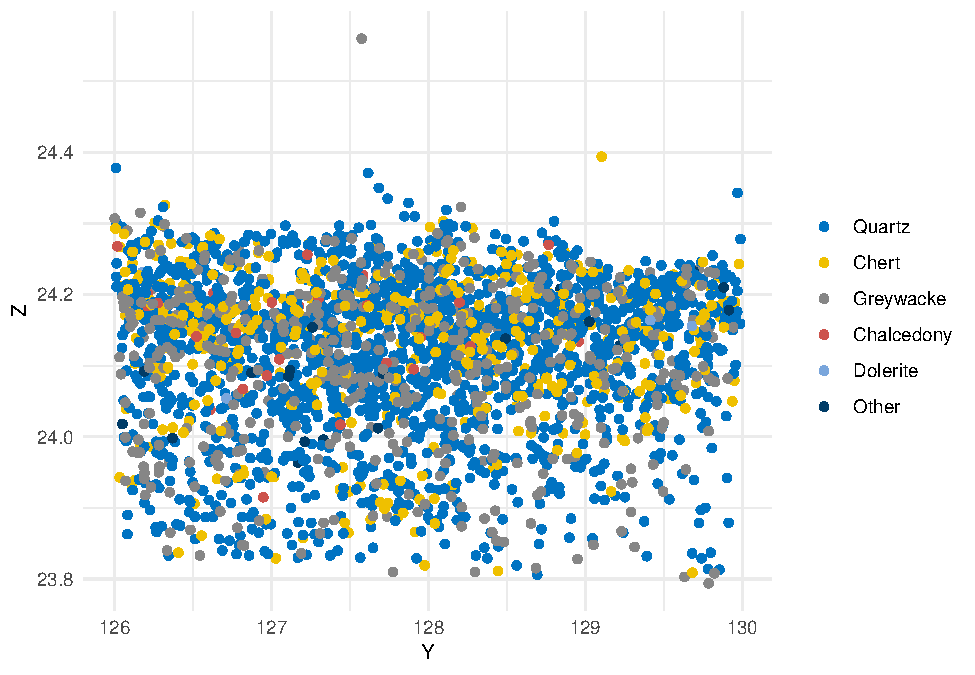
\includegraphics{thesis_files/figure-latex/spatialdistributionVB-1.pdf}
\caption{\label{fig:spatialdistributionVB}Spatial distribution of lithic artefacts (without chips) by raw material, on unit H.}
\end{figure}
However, when calculating the percentages of the three most important raw materials by cubic meter of excavated sediment (Figure \ref{fig:rmdispersion}) and plotting them by depth, there are significant differences in raw material distribution over time. From around 24.1 m of depth upwards, there is an important shift in quartz and chert frequencies, the latter increasing more than 10\%, and quartz dropping from c.~50\% to nearly 30\%. Greywacke frequencies follow those of quartz.

This shift seems to be associated with other significant changes in the Terrace sequence, such as the abovementioned increase in the amount of lithic materials in top Layer 5 and Layer 4e, but also the appearance of Vale Comprido technology. Additionally, these two moments are stratigraphically correlated with two different chronological horizons, the first, dated to c.~26 kcal BP, at c.~23.9 m depth, and associated with higher frequencies of quartz, and the second, dated to c.~24.7 kcal BP, at around 24.1 m depth, associated with higher frequencies of chert and a reduction in quartz presence.
\begin{verbatim}
`geom_smooth()` using method = 'loess' and formula 'y ~ x'
\end{verbatim}
\begin{figure}
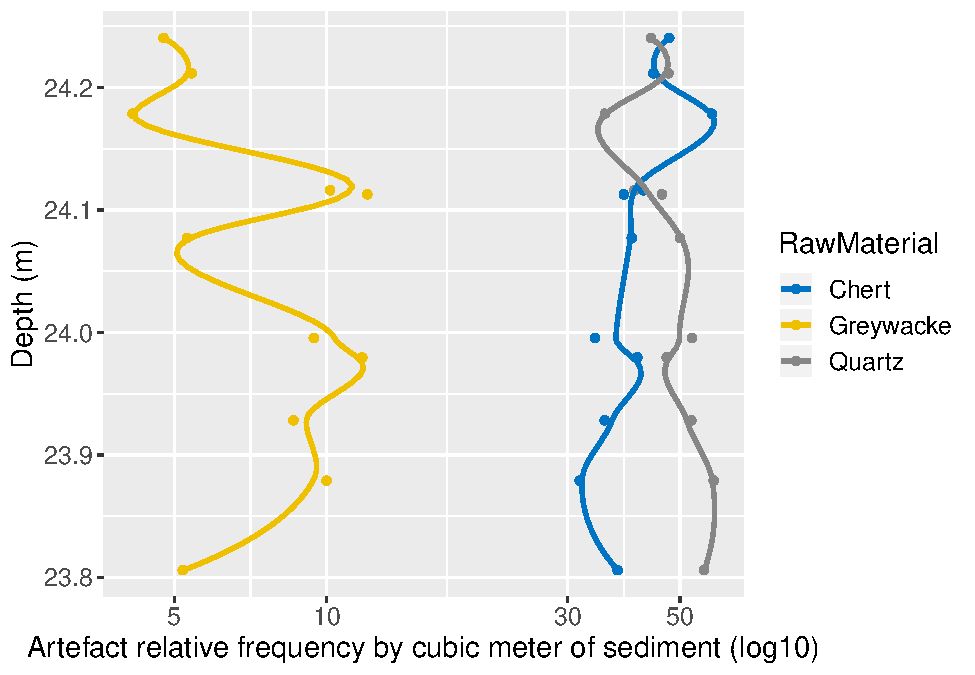
\includegraphics[width=1\linewidth]{thesis_files/figure-latex/rmdispersion-1} \caption{Raw material discard rates over time at Vale Boi. Each point is an excavation unit (spit). The lines are locally weighted regression lines (span ¼ 0.4) to aid in visualising the trend of increased discard in the upper part of the deposit.}\label{fig:rmdispersion}
\end{figure}
As such, and given the chronological, density of artifacts, and raw material preference patterns, it was decided that for this study the materials would be subdivided in two analytical units, to better understand any possible technological differences: \emph{Lower 5}, including all artifacts with Z values under 24.1; \emph{Upper 5/4E}, including all artifacts with Z values of 24.1 and above. The value 24.1 is arbitrary and was chosen for the reasons mentioned before: it seems to be where the separation between higher and lower densities of lithic materials occurs and, also, where the inversion of quartz and chert frequencies happens.

A total of 26711 pieces were analyzed for both groups, 11094 from Lower 5 group and 15609 for the Upper 5/4E. Most of these are chips (70.62\% from Lower 5 and 65.8\% from Upper 5/4E), followed by shatters, which make up c.~21\% and c.~24\% of the groups, respectively. These extremely high numbers for debris are mostly the result of quartz use, which can be explained not only by on-site knapping of this raw material but mostly by its breakage patterns (especially when coarser), which typically produces more waste than in other raw materials.

For Lower 5, cores and debitage products represent a cumulative frequency of c.~8\%. For Upper 5/4E, debitage products represent nearly 10\% of the group's assemblage. Complete blanks are the most represented class for both groups, with 1476 identified pieces, 4.5\% for Lower 5 and 6.18\% for Upper 5/4E, followed by blank fragments, with an absolute count of 248 for Lower 5 and 336 for Upper 5/4E. Cores are also relatively frequent within these assemblages, with an absolute count of 123 cores, 46 for Lower 5 and 77 for Upper 5/4E, while core fragments appear in much smaller numbers (n=11 and n=16, respectively).

During the analysis, 167 retouched pieces were identified, 55 on Lower 5, representing 0.5\% of the group, and 112 on Upper 5/4E, with a frequency of 0.72\%. Retouched piece fragments composed a much smaller number (n = 7 for Lower 5 and n = 16 for Upper 5/4E).
\begin{landscape}\begin{table}

\caption{\label{tab:general1}Technological class by raw material for Lower 5.}
\centering
\resizebox{\linewidth}{!}{
\begin{tabular}[t]{>{\bfseries}lrlrlrlrlrlrlrl}
\toprule
Class & Quartz (n) & Quartz (\%) & Chert (n) & Chert (\%) & Greywacke (n) & Greywacke (\%) & Dolerite (n) & Dolerite (\%) & Chalcedony (n) & Chalcedony (\%) & Other (n) & Other (\%) & Total & Total (\%)\\
\midrule
Anvil & 0 & 0\% & 0 & 0\% & 2 & 0.09\% & 0 & 0\% & 0 & 0\% & 0 & 0\% & 2 & 0.02\%\\
Blank & 281 & 3.58\% & 171 & 15.86\% & 44 & 2.08\% & 3 & 50\% & 6 & 37.5\% & 4 & 11.76\% & 509 & 4.59\%\\
BlankFrag & 132 & 1.68\% & 90 & 8.35\% & 23 & 1.09\% & 1 & 16.67\% & 1 & 6.25\% & 1 & 2.94\% & 248 & 2.24\%\\
Core & 18 & 0.23\% & 23 & 2.13\% & 3 & 0.14\% & 0 & 0\% & 1 & 6.25\% & 1 & 2.94\% & 46 & 0.41\%\\
CoreFrag & 2 & 0.03\% & 8 & 0.74\% & 0 & 0\% & 1 & 16.67\% & 0 & 0\% & 0 & 0\% & 11 & 0.1\%\\
\addlinespace
CorePreparProd & 1 & 0.01\% & 0 & 0\% & 0 & 0\% & 0 & 0\% & 0 & 0\% & 0 & 0\% & 1 & 0.01\%\\
Manuport & 0 & 0\% & 0 & 0\% & 2 & 0.09\% & 0 & 0\% & 0 & 0\% & 1 & 2.94\% & 3 & 0.03\%\\
RetouchedPiece & 15 & 0.19\% & 38 & 3.53\% & 1 & 0.05\% & 0 & 0\% & 1 & 6.25\% & 0 & 0\% & 55 & 0.5\%\\
RetouchedPieceFrag & 3 & 0.04\% & 4 & 0.37\% & 0 & 0\% & 0 & 0\% & 0 & 0\% & 0 & 0\% & 7 & 0.06\%\\
Shatter & 1754 & 22.36\% & 95 & 8.81\% & 507 & 23.96\% & 0 & 0\% & 5 & 31.25\% & 16 & 47.06\% & 2377 & 21.43\%\\
\addlinespace
Chip & 5638 & 71.88\% & 649 & 60.2\% & 1534 & 72.5\% & 1 & 16.67\% & 2 & 12.5\% & 11 & 32.35\% & 7835 & 70.62\%\\
Total & 7844 & - & 1078 & - & 2116 & - & 6 & - & 16 & - & 34 & - & 11094 & -\\
\bottomrule
\end{tabular}}
\end{table}
\end{landscape}
\begin{landscape}\begin{table}

\caption{\label{tab:general2}Technological class by raw material for Upper 5/4E.}
\centering
\resizebox{\linewidth}{!}{
\begin{tabular}[t]{>{\bfseries}lrlrlrlrlrlrlrl}
\toprule
Class & Quartz (n) & Quartz (\%) & Chert (n) & Chert (\%) & Greywacke (n) & Greywacke (\%) & Dolerite (n) & Dolerite (\%) & Chalcedony (n) & Chalcedony (\%) & Other (n) & Other (\%) & Total & Total (\%)\\
\midrule
Blank & 438 & 3.91\% & 407 & 19.53\% & 80 & 3.62\% & 14 & 60.87\% & 18 & 32.14\% & 8 & 34.78\% & 965 & 6.18\%\\
BlankFrag & 151 & 1.35\% & 155 & 7.44\% & 20 & 0.9\% & 3 & 13.04\% & 7 & 12.5\% & 0 & 0\% & 336 & 2.15\%\\
Burin spall & 0 & 0\% & 1 & 0.05\% & 0 & 0\% & 0 & 0\% & 0 & 0\% & 0 & 0\% & 1 & 0.01\%\\
Core & 32 & 0.29\% & 42 & 2.02\% & 1 & 0.05\% & 0 & 0\% & 0 & 0\% & 2 & 8.7\% & 77 & 0.49\%\\
CoreFrag & 4 & 0.04\% & 10 & 0.48\% & 0 & 0\% & 0 & 0\% & 0 & 0\% & 0 & 0\% & 14 & 0.09\%\\
\addlinespace
CorePreparProd & 1 & 0.01\% & 5 & 0.24\% & 0 & 0\% & 0 & 0\% & 0 & 0\% & 0 & 0\% & 6 & 0.04\%\\
Manuport & 0 & 0\% & 0 & 0\% & 5 & 0.23\% & 0 & 0\% & 0 & 0\% & 1 & 4.35\% & 6 & 0.04\%\\
RetouchedPiece & 34 & 0.3\% & 70 & 3.36\% & 2 & 0.09\% & 5 & 21.74\% & 1 & 1.79\% & 0 & 0\% & 112 & 0.72\%\\
RetouchedPieceFrag & 6 & 0.05\% & 9 & 0.43\% & 1 & 0.05\% & 0 & 0\% & 0 & 0\% & 0 & 0\% & 16 & 0.1\%\\
Shatter & 3006 & 26.81\% & 227 & 10.89\% & 563 & 25.46\% & 1 & 4.35\% & 15 & 26.79\% & 12 & 52.17\% & 3824 & 24.5\%\\
\addlinespace
Chip & 7540 & 67.25\% & 1158 & 55.57\% & 1539 & 69.61\% & 0 & 0\% & 15 & 26.79\% & 0 & 0\% & 10252 & 65.68\%\\
Total & 11212 & - & 2084 & - & 2211 & - & 23 & - & 56 & - & 23 & - & 15609 & -\\
\bottomrule
\end{tabular}}
\end{table}
\end{landscape}
\hypertarget{lapa-do-picareiro-2}{%
\subsection{Lapa do Picareiro}\label{lapa-do-picareiro-2}}

The materials from Lapa do Picareiro selected for this study come exclusively from Levels U and T. Based on chronological data and artifact distribution along the sequence, these levels had been previously organized into two distinct cultural horizons (Haws et al.~2019), somehow similar to the Terminal Gravettian and Proto-Solutrean phases in the traditional transition model (Zilhão et al.~1999).

Given this geo-archaeological background, for the present analysis the materials were separated into two assembllages: U/Lower T, which included all artifacts with depths inferior to 566.9 m or (in case of artifacts lacking 3D coordinates) from all spits from Level U and spits 6 through 8 from Level T (Haws et al.~2019); Middle T, including all artifacts with depths equal or superior to 566.9 m, or from the top five spits of Level T. Any other artifact in the assemblage which did not have a depth value or Level/Spit was not considered in these results since it lacked the needed information to contextualize its technological attributes. Also excluded from this study are the materials found on top of Level T undoubtedly attributed to the solutrean (Haws et al.~2019, Bennedeti et al.~2018).

A total of 376 pieces were analyzed, 196 coming from the U/Lower T phase and 180 from the Middle T group. In both phases, debitage waste is mostly composed of chips, which represents 49.4\% of the U/Lower T group and 37.2\% of the Middle T group. As in Vale Boi, these values for chippage can be mostly explained by quartz breakage patterns.

The second most present class for both assemblages are complete blanks, which represent 14.2\% of the U/Lower T group and 37.2\% of the Middle T group, followed by blank fragments (13.7\% and 15.5\%, respectively). Retouched pieces have relatively small frequencies, representing c.~3\% in both U/Lower T and Middle T. Cores are very scarce in both groups, 1\% in the U/Lower T group (n=2) and c.~3\% in the Middle T (n=5).
\begin{table}

\caption{\label{tab:generalTG}Technological class by raw material (U/Lower T phase).}
\centering
\resizebox{\linewidth}{!}{
\begin{tabular}[t]{>{\bfseries}lrlrlrlrl}
\toprule
Class & Quartz (n) & Quartz (\%) & Chert (n) & Chert (\%) & Other (n) & Other (\%) & Total & Total (\%)\\
\midrule
Blank & 30 & 20.83\% & 24 & 53.33\% & 1 & 14.29\% & 55 & 28.06\%\\
BlankFrag & 22 & 15.28\% & 4 & 8.89\% & 1 & 14.29\% & 27 & 13.78\%\\
Core & 2 & 1.39\% & 0 & 0\% & 0 & 0\% & 2 & 1.02\%\\
CorePreparProd & 0 & 0\% & 1 & 2.22\% & 0 & 0\% & 1 & 0.51\%\\
Manuport & 0 & 0\% & 0 & 0\% & 1 & 14.29\% & 1 & 0.51\%\\
\addlinespace
RetouchedPiece & 1 & 0.69\% & 5 & 11.11\% & 0 & 0\% & 6 & 3.06\%\\
Shatter & 4 & 2.78\% & 1 & 2.22\% & 2 & 28.57\% & 7 & 3.57\%\\
Chip & 85 & 59.03\% & 10 & 22.22\% & 2 & 28.57\% & 97 & 49.49\%\\
Total (RM) & 144 & - & 45 & - & 7 & - & 196 & -\\
\bottomrule
\end{tabular}}
\end{table}
\begin{table}

\caption{\label{tab:generalPR}Technological class by raw material (Middle T phase).}
\centering
\resizebox{\linewidth}{!}{
\begin{tabular}[t]{>{\bfseries}lrlrlrlrl}
\toprule
Class & Quartz (n) & Quartz (\%) & Chert (n) & Chert (\%) & Other (n) & Other (\%) & Total & Total (\%)\\
\midrule
Blank & 19 & 19\% & 46 & 63.01\% & 2 & 28.57\% & 67 & 37.22\%\\
BlankFrag & 19 & 19\% & 9 & 12.33\% & 0 & 0\% & 28 & 15.56\%\\
Core & 2 & 2\% & 2 & 2.74\% & 1 & 14.29\% & 5 & 2.78\%\\
RetouchedPiece & 0 & 0\% & 5 & 6.85\% & 0 & 0\% & 5 & 2.78\%\\
Shatter & 3 & 3\% & 2 & 2.74\% & 3 & 42.86\% & 8 & 4.44\%\\
\addlinespace
Chip & 57 & 57\% & 9 & 12.33\% & 1 & 14.29\% & 67 & 37.22\%\\
Total (RM) & 100 & - & 73 & - & 7 & - & 180 & -\\
\bottomrule
\end{tabular}}
\end{table}
\hypertarget{raw-materials}{%
\section{Raw materials}\label{raw-materials}}

Raw material use and availability, specifically abundance and quality, stand as important factors for understanding the organization of technology, as it may affect decisions regarding tool design and conservation of such tools (Andrefsky, 1994), as well as mobility and niche expansion (Cascalheira, 2013). This quality is connected to both the raw material's fracture mechanics and their intrinsic mineral characteristics, such as the size of their grain, homogeneity (Andrefsky, 1994), or even hardness (Kempson \& Wadley, 2011), which allow the knapper predictability over the outcome (Andresfsky 2005).

There are a number of stones that are constant throughout the stone age archaeological record for having the necessary properties described above. Stones or minerals characterized by high frequencies of silica, such as chert or quartz, allow for good fracture predictability, while other materials with less homogeneity may progressively result in less predictable characteristics (Andresfsky 2005). Thus, despite the raw material variability within the pre-historic archaeological record, linked to its availability and geomorphological contexts of the sites, the selection is often coherent regarding fracture mechanics, where predictable conchoidal fractures are preferred (Inizan, Reduron-Ballinger, Roche, \& Tixier, 1999; Tixier \& Inizian, 1980) (Andrefsky 2005).

This pattern is also observable at Vale Boi and Lapa do Picareiro as showned below. Previous studies have shown that throughout most levels of human occupation at both sites, chert, fine quartz and greywacke (in the case of Vale Boi) or Quartzite (in the case of Lapa do Picareiro) (all three characterized by conchoidal fracture, although greywacke is often coarse and more unpredictable) were the most frequently used (Bicho, Cascalheira, \& Marreiros, 2012; Cascalheira, 2010; Marreiros, 2009) (Pereira et al.~2016, Haws et al.~2019, Beneddeti et al.~2018). While at Vale Boi all the materials are available at a regional and local scale, at Lapa do Picareiro a more detailed analysis is needed to assess raw material provenance. Also, although the presence of the main raw materials is documented across all archaeological levels in Vale Boi, with each occupation differing in the frequency of their use, chert is always the primary material used for knapping (Cascalheira, 2010). At Lapa do Picareiro, the use of chert is not always a preference, such as in the case of Level FF, where quartzite is clearly dominant. The characteristics of Lapa do Picareiro and the potential functional specificities of each occupation must have had a significant impact on the type and quality of the discard materials.

For the present study, criteria used for raw material analysis focused on the identification of broader groups of stones and minerals, based on their general observable characteristics, without focusing on particular features within each raw material. Two exceptions were made, however. At both sites, quartz was subdivided into different categories regarding the size of the grain, to isolate and better understand the different uses of quartz over time. At Lapa do Picareiro, chert was organized based on color to evaluate the integrity of the deposits and, preliminarly, explore the spatial organization of levels U and T. Both of these exceptions are presented in the following sections where the patterns of exploitation of the more relevant raw materials are discussed for each site.

\hypertarget{vale-boi-3}{%
\subsection{Vale Boi}\label{vale-boi-3}}

One of the most relevant raw materials in both of Vale Boi analytical units used for this study is quartz (encompassing rock crystal, fine, medium and coarse qualities), which represents c.~43\% of the total assemblage for the Upper 5/4E group, and c.~51\% for Lower 5. Chert, on the other hand, represents c.~46\% of the Upper 5/4E phase and 38\% of the Lower 5. Finally, greywacke, dolerite, chalcedony, and other raw materials that due to their low frequencies were collapsed in the category ``Other'', together represent c.~11\% of both assemblages (Figure \ref{fig:rmvb}).
\begin{figure}
\centering
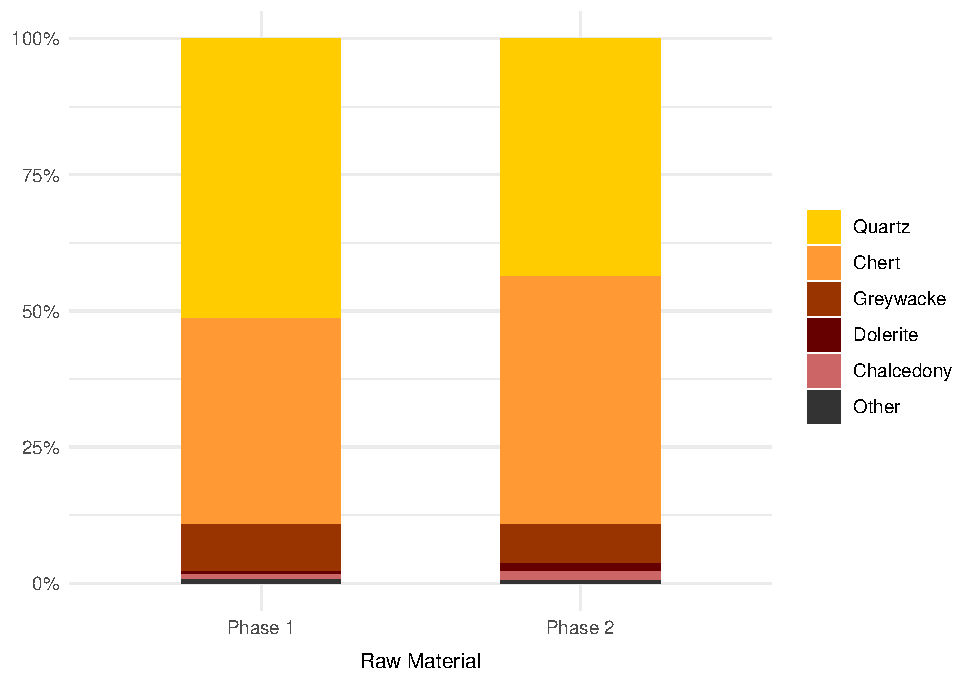
\includegraphics{thesis_files/figure-latex/rmvb-1.pdf}
\caption{\label{fig:rmvb}Vale Boi. Frequencies of raw materials by phase. Chips and shatters not included.}
\end{figure}
\hypertarget{quartz}{%
\subsubsection{Quartz}\label{quartz}}

The number of chips and shatter in quartz are, as seen in Table XXX, extremely high, both in its representativity within the raw material, with c.~94\% for both Lower 5 and Upper 5/4E, and when compared to the relative frequencies of other raw materials.

Despite the low frequencies presented on the table, there is a large number of quartz blanks (n=281 for Lower 5 and n=438 for Upper 5/4E) compared to the rest of the classes, as well as cores (n=18 for Lower 5 and n=32 for Upper 5/4E) and retouched pieces (n=15 for Lower 5 and n=34 for Upper 5/4E).
Most of the quartz artifacts do not show the presence of cortex, with nearly 95\% of all artifacts having 0\% cortex. When cortex is present, around 72\% of the artifacts indicate the exploitation of cobbles or pebbles. These patterns are similar for both Lower 5 and Upper 5/4E (Figure \ref{fig:quartzqualityVB}).

As mentioned before, quartz was organized into groups regarding grain size. Analyzing the artifact class frequency through the different identified types of quartz confirmed an already expected pattern: the production of blanks was largely accomplished using fine and medium quality quartz (52.1\% and 32.7\% for Lower 5, and 49.3\% and 32.1\% for Upper 5/4E, respectively). Most of the retouched tools were also recorded for these two types of quartz quality (66.7\% and 26.7\% for Lower 5, and 55.9\% and 44.1\% for Upper 5/4E). No retouched pieces were identified in coarse quartz and rock crystal. The latter type represents, also, a rather small fraction of the assemblage. In accordance with previous studies on Vale Boi lithic industries (e.g.~Cascalheira 2009, Marreiros 2009) coarse quartz appears mostly as knapping shatters, or as other type of fragments not related to human knapping (see Manne et al.~2012 for more information).
\begin{table}[!h]

\caption{\label{tab:quartzquality2}Vale Boi - Upper 5/4E. Frequencies of technological classes by quartz quality.}
\centering
\resizebox{\linewidth}{!}{
\begin{tabular}[t]{>{\bfseries}llllll}
\toprule
Quartz quality & Blank & Core & CorePreparProd & RetouchedPiece & Total\\
\midrule
QuartzQuality, n (\%) &  &  &  &  & \\
Coarse & 82 (18.7) & 9 (28.1) & 0 (0.0) & 0 (0.0) & 91 (18.0)\\
Fine & 223 (50.9) & 7 (21.9) & 0 (0.0) & 19 (55.9) & 249 (49.3)\\
Medium & 130 (29.7) & 16 (50.0) & 1 (100.0) & 15 (44.1) & 162 (32.1)\\
RockCrystal & 3 (0.7) & 0 (0.0) & 0 (0.0) & 0 (0.0) & 3 (0.6)\\
\bottomrule
\end{tabular}}
\end{table}
\hypertarget{chert}{%
\subsubsection{Chert}\label{chert}}

Chert shows high frequencies of blanks (15.8\% for Lower 5 and 19.5\% for Upper 5/4E) when compared to every other class, excluding chips (Table XXX). The latter represents more than 50\% of the chert assemblages, with an absolute frequency of 649 chips for Lower 5 and 1158 for Upper 5/4E.

Although chert shows smaller absolute numbers for blanks (n=171 for Lower 5 and n=407 for Upper 5/4E) and blank fragments (n=90 for Lower 5 and n=155 for Upper 5/4E) compared to quartz, there is a large quantity of cores representing 2.1\% of total chert in Lower 5 and 2\% in Upper 5/4E. However, Table XXX shows a noticeable difference in the ratio between chert blanks and quartz blanks in Lower 5 and Upper 5/4E, with the latter showing a higher frequency of chert blanks compared to Upper 5/4E.

Regarding retouched pieces, these represent more than 3\% of chert for both phases, a number far higher than those in other raw materials, thus showing that chert, although less present than quartz in blanks (although barely in Upper 5/4E), might have been preferentially used for formal tool production.

Chert also shows the most prominent variability of cortex frequencies in both phases (Figure @(fig:rmcortex)), although there is a clear dominance of artifacts with 0\% cortex, a pattern that was already expected, following the process of the knapping sequence, where only the first blanks removed from an unmodified block will be entirely cortical, showing increasingly less cortex for posterior removals (Andrefsky 2005). It is noteworthy, however, that for both phases, a significant number of chert artifacts (c.~25\%) presented cortical surfaces, confirming that chert nodules were imported to the site and thus all phases of the reduction sequences are likely represented.

This variability in cortex presence is accompanied by some diversity of cortex types, with the presence of both cobble and outcrop sources, even though for almost 85\% of the artifacts it was not possible to identify a specific type of cortex (Table \ref{tab:cortextab1}).

\hypertarget{greywacke}{%
\subsubsection{Greywacke}\label{greywacke}}

Greywacke is a variety of sandstone, often characterized by its hardness, dark color and poorly sorted grains of quartz and feldspar (Haldar and Tisljar 2014). At Vale Boi, this raw material is highly heterogeneous, showing a wide variety of grain sizes and colors.

Within the studied assemblage, greywacke is best represented by debitage waste, with nearly 25\% of shatter and around 70\% of chips, for both Lower 5 and Upper 5/4E. In contrast, relatively low numbers for blanks (n=44 for Lower 5 and n=80 for Upper 5/4E) and cores (n=3 for Lower 5 and 1 for Upper 5/4E) were recorded. The same applies to the retouched tools category, with three artifacts recorded, one of which is a Vale Comprido piece, in the Upper 5/4E phase.

When chips and shatters are removed, greywacke has a representation of less than 10\% in both assemblages making it the third most used raw material.

Similarly to the other raw materials, there is, for both phases, the predominance of debitage without cortex (Figure \ref{fig:rmcortex}). There is, however, some variability in cortex presence, even if in smaller frequencies than the patterns observed for chert. As in the case of quartz, most of the identified cortex presented water-worned surfaces, indicating the exploitation of cobbles or, most likely, slabs.

\hypertarget{dolerite}{%
\subsubsection{Dolerite}\label{dolerite}}

Dolerite is a volcanic igneous rock, occurring mostly in dikes, varying between coarse and fine textures, and often having a dark, grey or greyish-green coloration (Haldar and Tisljar 2014; Wadley and Kempson 2011; Belmiro 2018). In the Algarve, its presence is registered in two main areas : , and near Sagres, southwest of the Algarve, as outcrops within the Messejana fault (Belmiro 2018).

At Vale Boi, this raw material was first identified as jasper when excavating the levels referring to the Proto-Solutrean occupation in the terrace area (units J-L), before 2012 (Marreiros 2009). The material has a very characteristic reddish-brown color and fine texture, with a conchoidal fracture. Despite this coloration, which is also present in jasper, a red-colored variety of chalcedony, the raw material was later identified as dolerite, and its coloration explained by the presence of a reddish patina which would have altered the original rock by processes of iron mineral oxidation through contact with the terra rossa (Belmiro 2018).

The analysis of a thin section obtained from a dolerite fragment from the present assemblage allowed the characterization of this raw material, through its visible features and petrography.

The reddish coloration was confirmed to be an exterior patina, no more than 1 mm thick, completely covering the artifacts. The actual rock still displays a fine texture but with an opaque black color.

Results from the petrographic analysis done through the observation of the thin section using a polarizing microscope revealed the presence of several minerals, such as feldspar, plagioclase, quartz, small quantities of silica, little presence of mica and iron oxide, which are in concordance with the mineral composition of dolerite or possibly hornfels (Wadley and Kempson 2011). The feldspar minerals showed the presence of undulatory extinction, a deformation that takes place whenever certain minerals are exposed to high temperatures (Frost and Frost 2014), thus indicating that the raw material is highly metamorphized.

Regarding the differentiation between dolerite and hornfels, although these two rocks have different origins, the latter being of volcanic igneous origin, considered a contact metamorphic rock (Haldar and Tisljar 2014), they share enough physical and mineral characteristics (whenever the dolerite has a fine texture) to hinder their precise identification. Literature most often uses other methods to differentiate them, such as FTIR, XRF, by understanding not the mineral composition (which is essentially the same) but the ratio of components presence. This matter is further complexified by understanding that hornfels might originate from metamorphized igneous rocks, several sources of hornfels attributed to dolerite dikes (Wadley and Kempson 2011; Hallinan and Shaw 2017).

Given this difficulty, although the present analysis will use the term dolerite, for their reported similarities in terms of texture, grain size and fracture, further chemical studies need to be done in order to confirm whether the raw material is dolerite or possibly hornfels. Regarding the latter, there is also the presence of hornfels outcrops and rounded pebbles in the Algarve, near the southwestern coast, thus strengthening the hypothesis that this raw material, whether dolerite or hornfels, is available regionally.

Looking at the interior of dolerite allowed, during the second moment of analysis, to identify other products in the same raw material, which were not previously identified due to the lack of the same reddish patina. This patina also appears throughout the assemblage, mostly on greywacke, although without forming the same 1 mm thick layer visible on the dolerite pieces. This may be explained by the inherent mineral characteristics of this type of raw material and their reaction with the surrounding sediment.

The presence of this patina in several degrees of intensity, preferentially in dolerite and greywacke, its presence in both finished complete artifacts and flake fragments or shatters, and its occurrence also reported in the literature as a process frequently affecting raw materials like hornfels (e.g., Hallinan and Shaw 2017), suggests that it is, in fact, the result of geological and chemical processes affecting these raw materials. Its absence from other raw materials, like chert or quartz, may reflect the inherent mineral properties of these materials.

Dolerite is a rather unusual raw material in the site of Vale Boi, appearing only in layers 4E and 5 of the Terrace and Proto-Solutrean levels of the Slope area. The most striking characteristic of this raw material in the assemblages under study is the low presence of chips or shatter (n=1 each), but high frequencies of blanks (50\% in Lower 5 and 60.8\% in Upper 5/4E) and blank fragments (16.6\% in Lower 5 and 13\% in Upper 5/4E) (Table XXX). Unlike Lower 5, in Upper 5/4E dolerite is represented by five retouched tools, some of which are Vale Comprido points. This raw material seems to have been used preferentially at Vale Boi for the production of these types of points, a pattern already observed in previous works (Marreiros 2009), where three out of five Vale Comprido points were identified as dolerite (originally jasper).

The absence of cores, with only one core fragment identified in the Lower 5 group, and low quantity of debitage waste may be explained by the importation of finished pieces or blanks to the site, suggesting that, most likely, no knapping activities occurred with this raw material at the site. This interpretation is, however, truncated by this study's phase analysis. As the identification of the inner aspect of dolerite was only achieved at the start of the second phase, which as referred before, consisted of the analysis of all cores and debitage products with a more complete database, shatter and chips were not revisited, thus not allowing for the possible identification of possible unpatinated dolerite within those classes, which might have been mistaken for fine-grained greywacke. This caveat does not, however, seem to influence the patterns regarding blank and retouched tools frequency.

\hypertarget{chalcedony}{%
\subsubsection{Chalcedony}\label{chalcedony}}

Chalcedony is a type of cryptocrystalline quartz, characterized by a waxy and glossy appearance, ranging from a variety of possible colors (Haldar and Tisljar 2014), although white is the only present variety in the studied assemblages. The chalcedony in levels 4E and 5 is also characterized by the frequent presence of inclusions, making this raw material poorly homogeneous.

Results indicate it may have been mainly used for the production of blanks, which represent 37.5\% of chalcedony in Lower 5 and 32.1\% in Upper 5/4E, with a rather small representation of retouched pieces (n=2), which include a Vale Comprido point in the Upper 5/4E group. The presence of a core in Lower 5, as well as the presence of shatter and chips (in small numbers - n\textless5 each for Lower 5 and n=15 each for Upper 5/4E) may indicate, contrary to the dolerite, onsite knapping of this raw material (Table XXX).

Compared to other raw materials, chalcedony has the lowest frequencies of cortex, in both phases, with almost 100\% of all artifacts (except shatter and chips) having 0\% cortex (Figure \ref{fig:rmcortex}).
\begin{figure}
\centering
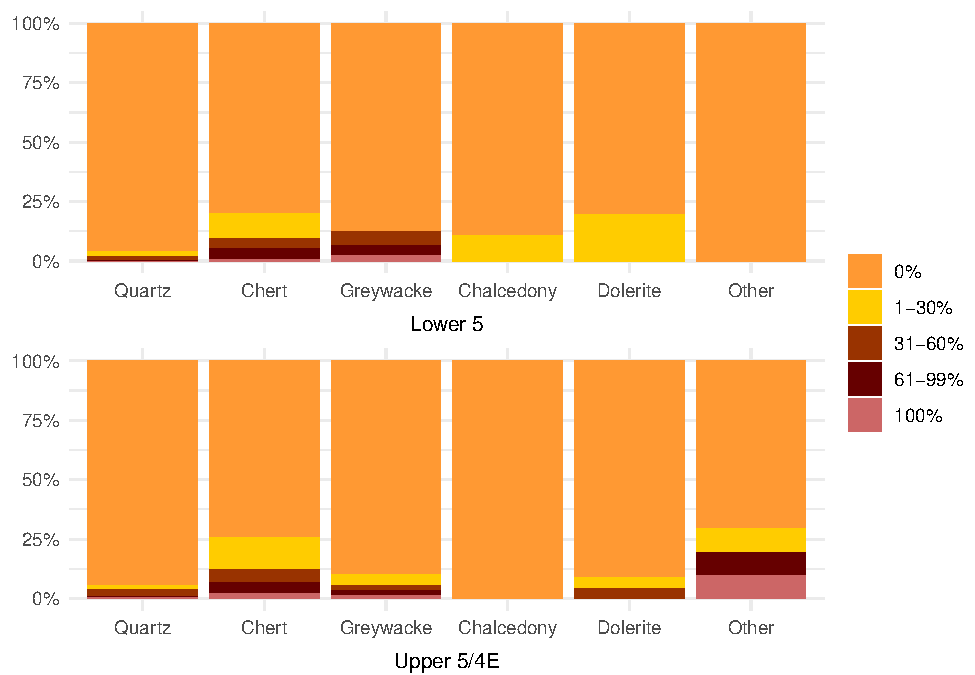
\includegraphics{thesis_files/figure-latex/rmcortex-1.pdf}
\caption{\label{fig:rmcortex}Vale Boi. Frequencies of cortex by raw material and phase. Chips and shatters not included.}
\end{figure}
\begin{table}

\caption{\label{tab:cortextab1}Vale Boi - Lower 5. Frequencies of cortex type by raw material.}
\centering
\resizebox{\linewidth}{!}{
\begin{tabular}[t]{>{\bfseries}lllll}
\toprule
Cortex attributes & Quartz & Chert & Greywacke & Total\\
\midrule
CortexType, n (\%) &  &  &  & \\
Cobble & 15 (83.3) & 5 (8.5) & 7 (77.8) & 27 (31.0)\\
Indeterminate & 2 (11.1) & 50 (84.7) & 0 (0.0) & 53 (60.9)\\
Outcrop & 1 (5.6) & 4 (6.8) & 2 (22.2) & 7 (8.0)\\
\bottomrule
\end{tabular}}
\end{table}
\begin{table}

\caption{\label{tab:cortextab2}Vale Boi - Upper 5/4E. Frequencies of cortex typeby raw material.}
\centering
\resizebox{\linewidth}{!}{
\begin{tabular}[t]{>{\bfseries}lllllll}
\toprule
Cortex attributes & Quartz & Chert & Greywacke & Dolerite & Other & Total\\
\midrule
CortexType, n (\%) &  &  &  &  &  & \\
Cobble & 30 (81.1) & 11 (6.7) & 9 (81.8) & 2 (100.0) & 3 (100.0) & 55 (25.3)\\
Indeterminate & 4 (10.8) & 123 (75.0) & 2 (18.2) & 0 (0.0) & 0 (0.0) & 129 (59.4)\\
Outcrop & 3 (8.1) & 30 (18.3) & 0 (0.0) & 0 (0.0) & 0 (0.0) & 33 (15.2)\\
\bottomrule
\end{tabular}}
\end{table}
\hypertarget{lapa-do-picareiro-3}{%
\subsection{Lapa do Picareiro}\label{lapa-do-picareiro-3}}

Comparatively to Vale Boi, Lapa do Picareiro shows less raw material variability, which might be explained by the lithological characteristics of the area, already explored in other studies that showed similar raw material presence patterns (Almeida, 2000; Zilhão, 1997), but can also be related to the location of the site in a high altitude environment with significant implications to the functional nature of the occupations (see Cascalheira and Bicho 2017). The main raw materials identified were quartz and chert (Figure \ref{fig:rmlp}). Quartz is dominant in the U/Lower T phase, representing c.~60\% of the assemblage, while chert is dominant in the Middle T phase, representing c.~59\%. The sporadic occurrence of other raw materials is the result of the identification of some quartzite artifacts on both phases.
\begin{figure}
\centering
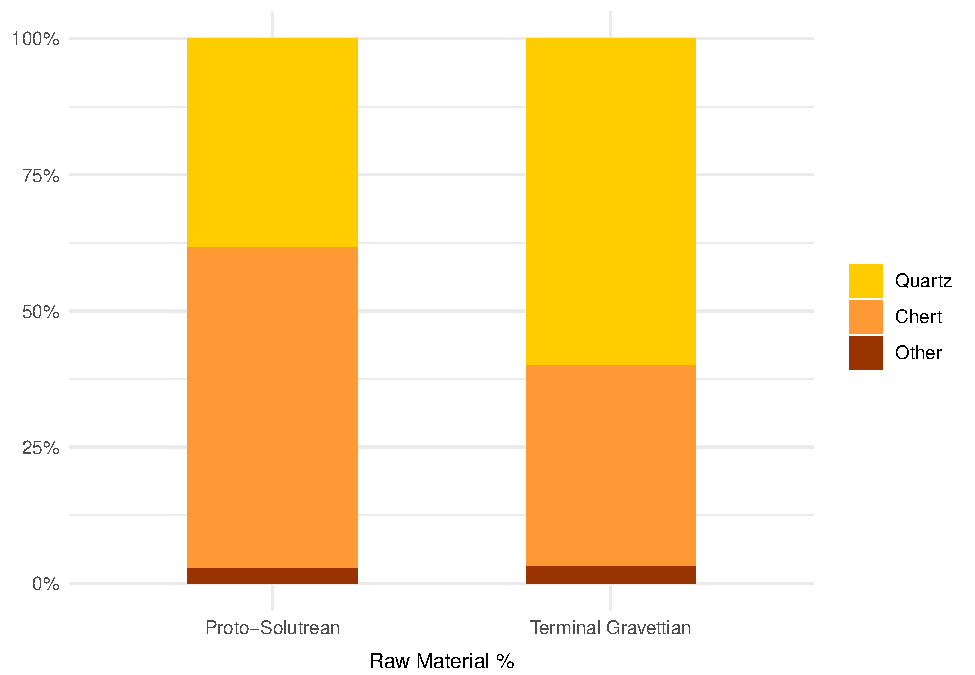
\includegraphics{thesis_files/figure-latex/rmlp-1.pdf}
\caption{\label{fig:rmlp}Lapa do Picareiro. Frequencies of raw material by phase. Chips and shatters not included.}
\end{figure}
\hypertarget{quartz-1}{%
\subsubsection{Quartz}\label{quartz-1}}

The number of chips in quartz, as seen on Table XXX, is extremely high, representing nearly 60\% of this raw material in both phases. Other waste products, i.e.~shatters, show much smaller numbers (n=4 for U/Lower T and n=3 for Middle T). Comparatively, complete blanks are the second most present class in quartz, with a frequency of 20\% (n=30) for the U/Lower T group, followed by blank fragments which represent 15.2\% of that assemblage. For the Middle T group, complete blanks and blank fragments show similar frequencies, representing c.~19\% each. Although in small numbers, quartz shows the highest number of cores (n=4, 2 in each group) from all raw materials, but a small number of retouched tools (n=1).

Regarding cortex, quartz shows frequencies as low as 6\% for cortex presence on the U/Lower T group, 12.5\% on the Middle T, being mostly composed of pieces with no cortex on their dorsal surfaces. When present, cortical surfaces are all water-worned, indicating the exploitation of cobbles/pebbles (Tables \ref{Tab:cortextabtg} and \ref{tab:cortextabpr}).

As in Vale Boi, quartz was categorized regarding grain quality and color (Tables @ref(tab:quartzqualityTG and \ref{tab:quartzqualityPR}. For both the U/Lower T group and Middle T, it is possible to observe a majority of fine quality quartz and rock crystal for both cores and blanks, with barely any presence of medium and coarse quality quartz. The latter category is completely absent in the Middle T group. One observable difference between the two groups is in the percentages of rock crystal and fine quality: in the U/Lower T, fine quality quartz represents c.~56\% of quartz, while rock crystal has a frequency of nearly 41\%; for Middle T, these percentages change, as fine quality quartz represents c.~38\%, against c.~57\% of rock crystal. Finally, the single identified retouched tool in U/Lower T was made in fine quality quartz.
\begin{table}

\caption{\label{tab:quartzqualityPR}Lapa do Picareiro - Middle T. Frequencies of technological classes by quartz quality.}
\centering
\resizebox{\linewidth}{!}{
\begin{tabular}[t]{>{\bfseries}llll}
\toprule
Quartz quality & Blank & Core & Total\\
\midrule
QuartzQuality, n (\%) &  &  & \\
Fine & 7 (36.8) & 1 (50.0) & 8 (38.1)\\
Medium & 1 (5.3) & 0 (0.0) & 1 (4.8)\\
RockCrystal & 11 (57.9) & 1 (50.0) & 12 (57.1)\\
\bottomrule
\end{tabular}}
\end{table}
\hypertarget{chert-1}{%
\subsubsection{Chert}\label{chert-1}}

Chert is characterized by a high frequency of complete blanks (c.~53\% for U/Lower T and c.~63\% for Middle T), with frequencies of c.~24\% and c.~15\% for chips and shatters in the U/Lower T and Middle T phases, respectively (Table XXX). Blank fragments are poorly represented comparatively to quartz, with an absolute count of four elements for U/Lower T and nine for the Middle T phase, representing c.~9\% and c.~12\% of the whole chert assemblage. Although there are few cores (n=2), retouched pieces have a relatively high frequency within chert (c.~11\% on U/Lower T and c.~7\% on Middle T) but also across all materials, suggesting that chert was preferentially used for the manufacture of formal tools.

Regarding cortex, chert shows mostly non-cortical pieces, particularly in the Middle T group where only 0\% or 1-30\% cortex frequencies were detected (Figure \ref{fig:cortexlp}). The low frequencies of cortex resulted in a low rate of identification of cortex types across the assemblage. In fact, only two pieces for U/Lower T phase allowed to track its provenience to an outcrop source (Tables \ref{tab:cortextabtg} and \ref{tab:cortextabpr}).

Although chert was not initially subdivided regarding its visible characteristics, throughout the analysis, it became apparent that there were several groups with identical colors and grains, which might have belonged to the same nodule. As such, these groups were posteriorly individualized, adding a variable to the database called ``ChertType'' which included codes for each identified type of chert, whose description is presented in Table \ref{tab:cherttable}.
\begin{table}

\caption{\label{tab:cherttable}Identified chert types. Description is mostly based on colour patterns, following the Munsel manual of color chart (Munsel Color (Firm) 2010).}
\centering
\begin{tabular}[t]{>{\bfseries}l>{\raggedright\arraybackslash}p{10cm}}
\toprule
Chert Type & Description\\
\midrule
RM1 & Fine grain, 2.5Y 7/6 and 6/6 (yellow and olive yellow) translucent color with opaque smoke-like patterns.\\
RM2 & Mostly 5YR 4/2 (dark reddish gray) and 4/3 (reddish brown) colouration, with 1mm 10YR 7/3 (very pale brown) dots and bigger 0.5 to 1 mm circular 10YR 7/2 (light gray) inclusions with coarser texture.\\
RM3 & Coarser texture, with veins and fog-like patterns with colour mix of 10YR 8/3, 7/3 (very pale brown), 7.5YR 7/3 (pink), 5YR 7/4 (pink) and 10YR 5/3 brown.\\
RM4 & Mostly 2.5Y 8/1 (white) with interior translucent areas.\\
RM5 & 2.5Y 6/2 (light brownish gray), closer to cortex 10YR 8/2 and 8/3 (very pale yellow) with circular 0.5 mm marks of 10YR 7/2 /(light gray) and 5Y 5/1 (gray) dots.\\
\addlinespace
RM6 & 10YR 8/3 (very pale brown) on borders, center fog-like pattern with mix of 10YR 4/2,3/3 (dark brown), 2.5Y 6/3 (light yellowish brown) and 5/1 (gray).\\
RM7 & Stripped-like ondulating pattern with several tonalities: 5YR 7/3, 8/3 (pink), 6/6 (reddish yellow), 7/1 (light gray), with certain areas with 7.5YR 7/8 (reddish yellow).\\
\bottomrule
\end{tabular}
\end{table}
After the classification of the chert types, it was attempted to refit the pieces in each group, but due to the high level of modification/edge damage of each piece and the fragmentation of the reduction sequences, no reffits were possible. Additionally, using the spatial information of artifact distribution, each group was plotted in order to understand any spatial restriction or relationship that could help to identify specific clusters throughout the stratigraphy (Figure \ref{fig:chertspatial}).

Most groups seem to show no particular spatial constraint or pattern when plotted. The exception are RM1 and RM6 that seem to have a significant concentration of materials, both around the 567 m of depth, which corresponds to the second spit of what is considered the Middle T phase, matching also with the highest quantity of chert in the whole stratigraphic sequence, and potentially indicating the isolation of that section of the sequence as a particularly undisturbed occupation episode. Further analyses will be, however, needed to better understand the meaning of clusters like these inside the cave.
\begin{figure}
\centering
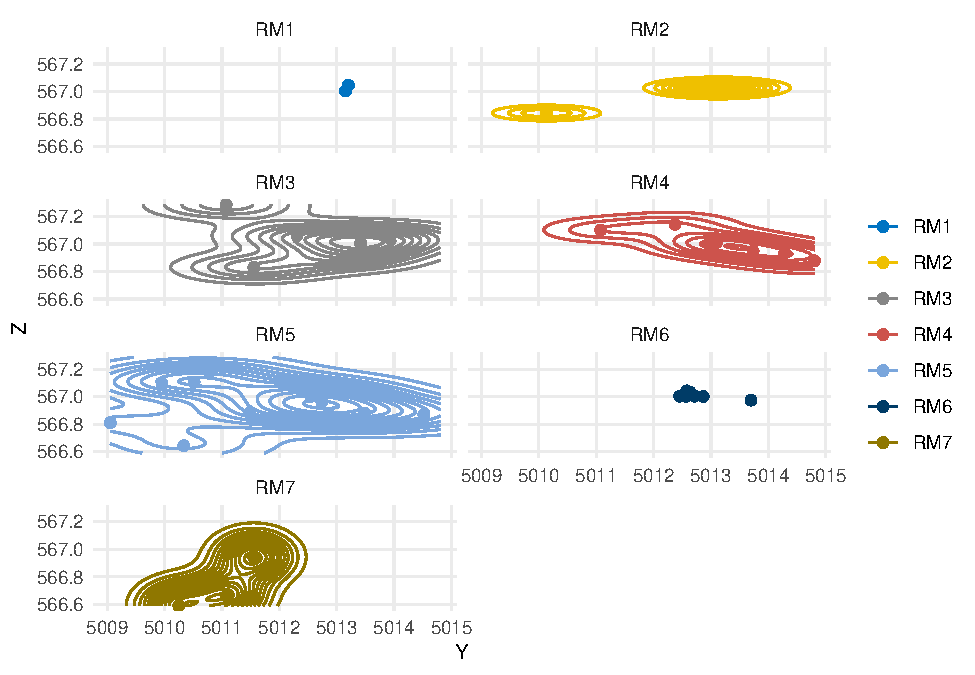
\includegraphics{thesis_files/figure-latex/chertspatial-1.pdf}
\caption{\label{fig:chertspatial}Spatial dispersion (Z vs Y) by chert type using total station data (countors represent a 2D Kernel density estimation).}
\end{figure}
\begin{figure}
\centering
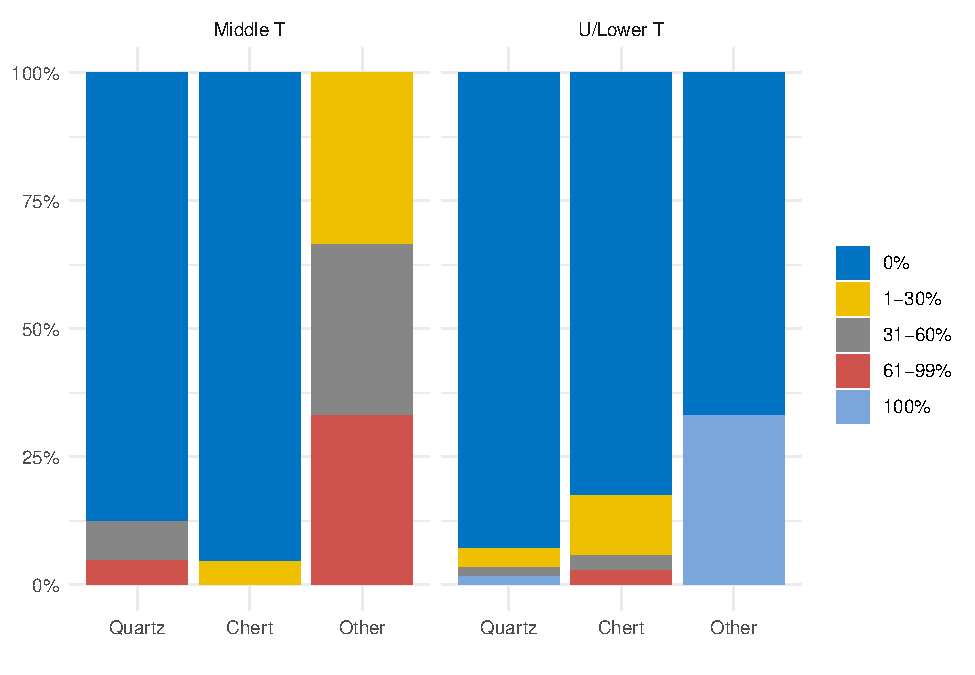
\includegraphics{thesis_files/figure-latex/cortexlp-1.pdf}
\caption{\label{fig:cortexlp}Lapa do Picareiro. Frequencies of cortex by raw material and by phase. Chips and shatters not included}
\end{figure}
\begin{table}

\caption{\label{tab:cortexabtg}Lapa do Picareiro - U/Lower T. Frequencies of cortex type by raw material.}
\centering
\resizebox{\linewidth}{!}{
\begin{tabular}[t]{>{\bfseries}llll}
\toprule
Cortex attributes & Quartz & Chert & Total\\
\midrule
CortexType, n (\%) &  &  & \\
Cobble & 3 (75.0) & 0 (0.0) & 5 (41.7)\\
Indeterminate & 1 (25.0) & 4 (66.7) & 5 (41.7)\\
Outcrop & 0 (0.0) & 2 (33.3) & 2 (16.7)\\
\bottomrule
\end{tabular}}
\end{table}
\begin{table}

\caption{\label{tab:cortextabpr}Lapa do Picareiro - Middle T. Frequencies of cortex type by raw material.}
\centering
\resizebox{\linewidth}{!}{
\begin{tabular}[t]{>{\bfseries}lllll}
\toprule
Cortex attributes & Quartz & Chert & Other & Total\\
\midrule
CortexType, n (\%) &  &  &  & \\
Cobble & 5 (100.0) & 0 (0.0) & 2 (66.7) & 7 (63.6)\\
Indeterminate & 0 (0.0) & 3 (100.0) & 1 (33.3) & 4 (36.4)\\
\bottomrule
\end{tabular}}
\end{table}
\hypertarget{technological-analysis}{%
\section{Technological analysis}\label{technological-analysis}}

\hypertarget{cores}{%
\subsection{Cores}\label{cores}}

\hypertarget{vale-boi-4}{%
\subsubsection{Vale Boi}\label{vale-boi-4}}

The core assemblage from Vale Boi totals 123 pieces, with 46 total pieces coming from the Lower 5 levels, and 77 from the Upper 5/4E group (Table XXX).

Excluding inform cores, which were not considered here because they do not possess all the recordable attributes, there is a clear dominance of single platform cores, for most raw materials and in both phases. Chert presents the highest variability of core types. In the Lower 5 group chert unidirectional prismatic cores are more frequent, while in the Upper 5/4E chert all core types are more evenly present.

Most of the cores were used for the extraction of flakes, although blade and bladelet scars also show relatively high frequencies associated with the exploitation of unidirectional prismatic cores in Lower 5 and Upper5/4E groups (Figure \ref{fig:coretypeVB}).
\begin{figure}
\centering
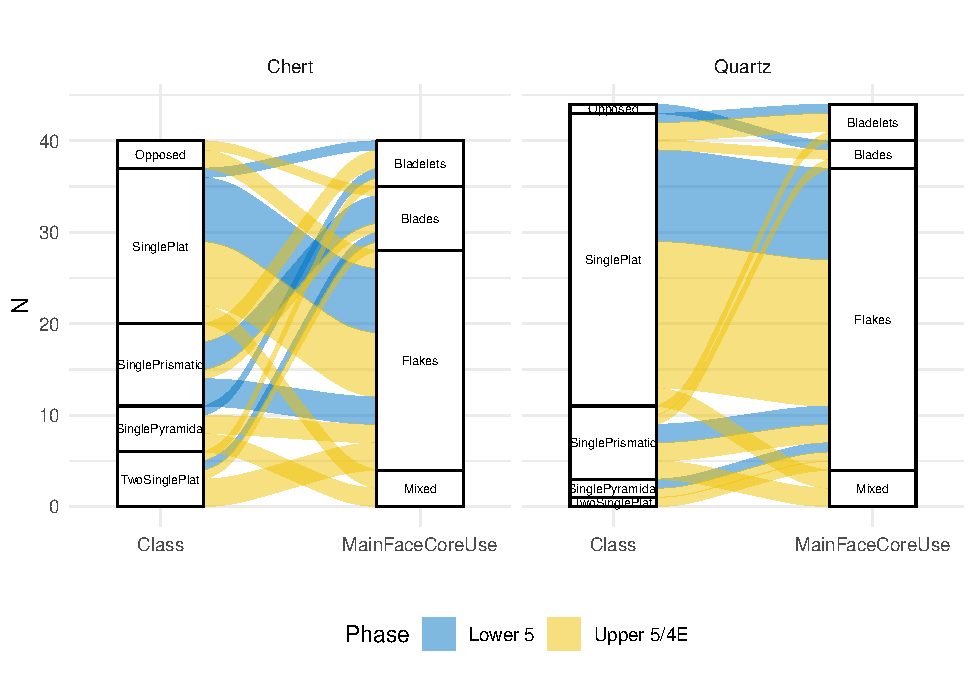
\includegraphics{thesis_files/figure-latex/coretypeVB-1.pdf}
\caption{\label{fig:coretypeVB}Vale Boi. Interaction of core type with type of extracted products by raw material and phase.}
\end{figure}
\begin{verbatim}

    F test to compare two variances

data:  CoreElongation by Phase
F = 0.54919, num df = 15, denom df = 26, p-value = 0.227
alternative hypothesis: true ratio of variances is not equal to 1
95 percent confidence interval:
 0.2301034 1.4712539
sample estimates:
ratio of variances 
         0.5491891 
\end{verbatim}
\begin{verbatim}
[1] 0.498451
\end{verbatim}
\begin{verbatim}

    F test to compare two variances

data:  CoreElongation by Phase
F = 2.2382, num df = 14, denom df = 28, p-value = 0.06766
alternative hypothesis: true ratio of variances is not equal to 1
95 percent confidence interval:
 0.9426702 6.1521489
sample estimates:
ratio of variances 
          2.238229 
\end{verbatim}
\begin{verbatim}
[1] 0.3166799
\end{verbatim}
\begin{verbatim}

    F test to compare two variances

data:  CoreFlattening by Phase
F = 1.0758, num df = 15, denom df = 26, p-value = 0.8422
alternative hypothesis: true ratio of variances is not equal to 1
95 percent confidence interval:
 0.4507464 2.8820186
sample estimates:
ratio of variances 
          1.075799 
\end{verbatim}
\begin{verbatim}
[1] 0.847313
\end{verbatim}
\begin{verbatim}

    F test to compare two variances

data:  CoreFlattening by Phase
F = 3.1072, num df = 14, denom df = 28, p-value = 0.01034
alternative hypothesis: true ratio of variances is not equal to 1
95 percent confidence interval:
 1.308645 8.540612
sample estimates:
ratio of variances 
          3.107182 
\end{verbatim}
\begin{verbatim}
[1] 0.2651861
\end{verbatim}
Most of the analyzed core platforms are plain or cortical. On Upper 5/4E there is a small frequency of faceted platforms on both quartz and chert (3\% and 18.5\% respectively). Platforms width and thickness means show smaller platforms for chert on both phases, while greywacke shows the highest means for platform measurements (Table XXX). This pattern is similar for other measurements, for which chert and quartz exhibit the smaller means.

Regarding elongation, Figure \ref{fig:coreboxplotVB} shows wider range and higher elongation values for chert cores in both phases. Upper 5/4E seems to have less elongated cores in both chert and quartz, but the t-test results indicate no significant difference between the sets (Chert p-value = 0.498451, Quartz p-value = 0.3166799. Other raw materials, including greywacke, show the lower values for elongation.

Core flattening (Figure \ref{fig:coreboxplotVB}) (calculated by dividing maximum width by thickness) reveals that greywacke and other raw materials show higher values, while quartz and chert cores have similar values for both phases (Chert t-test p-value = 0.847313, Quartz t-test p-value = 0.2651861), with flattening median values of around 1.5, centered in between the second and third quartiles of the distribution.
\begin{figure}
\centering
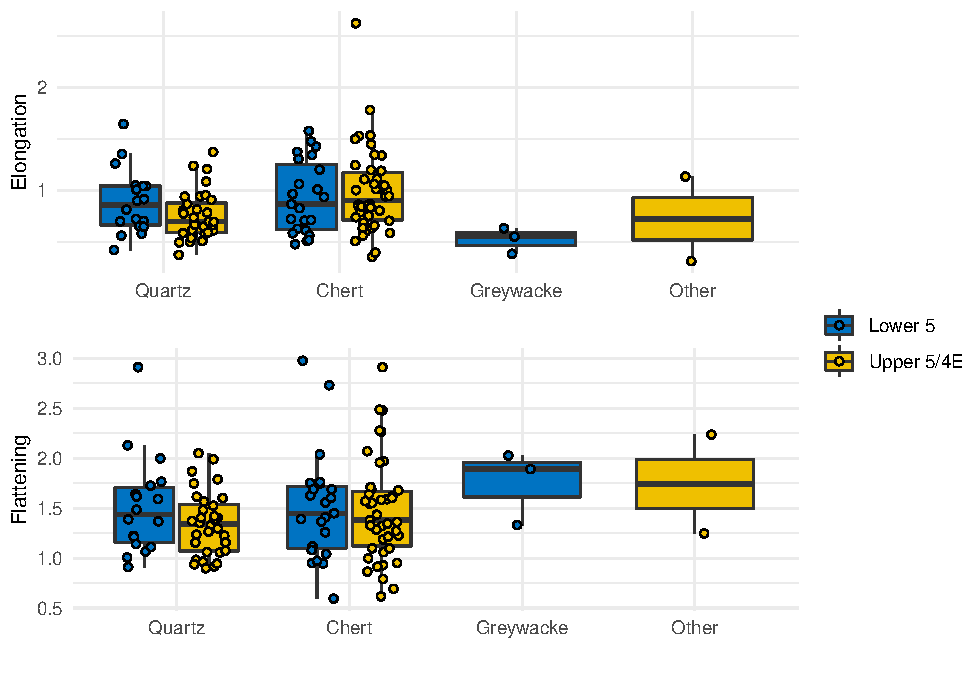
\includegraphics{thesis_files/figure-latex/corebloxplotVB-1.pdf}
\caption{\label{fig:corebloxplotVB}Vale Boi. Boxplots of core elongation and flattening by raw material and phase.}
\end{figure}
\hypertarget{lapa-do-picareiro-4}{%
\subsubsection{Lapa do Picareiro}\label{lapa-do-picareiro-4}}

A total of seven cores were recorded on the Lapa do Picareiro assemblages, two in the U/Lower T group and five in the Middle T, of which two are in chert and two are in quartz.

Single platform, prismatic and pyramidal cores were identified in the Middle T group. These were mainly used to remove flakes (Figure \ref{fig:coretypeLP}) and only prismatic cores showed evidence for the production of mixed blanks. Platforms tend to be unfacetted, although a small number of cores presented dihedral platforms. The number of debitage surfaces is greater on chert cores for the Middle T group, while quartz varies between single and three faces (Table XXX).

Metrically, chert has smaller mean values for all core measurements when compared to other raw materials, showing, however, higher elongation ratios (Figure \ref{fig:coreboxplotLP}). Regarding quartz cores, the differences between the U/Lower T phase and the Middle T phase are very obvious, with the first group showing more elongated cores with low flattening values. These differences may simply be the result of the rather small number of cores present in the assemblage and a consequent low intra-assemblage variability.
\begin{figure}
\centering
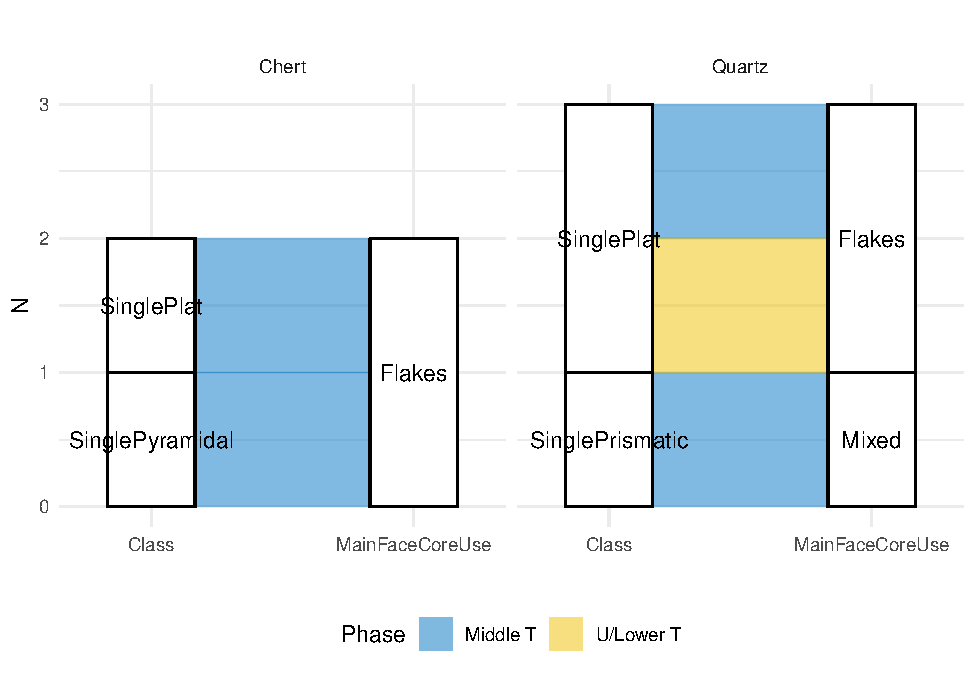
\includegraphics{thesis_files/figure-latex/coretypeLP-1.pdf}
\caption{\label{fig:coretypeLP}Vale Boi. Interaction of core type with type of extracted products by raw material and phase.}
\end{figure}
\begin{figure}
\centering
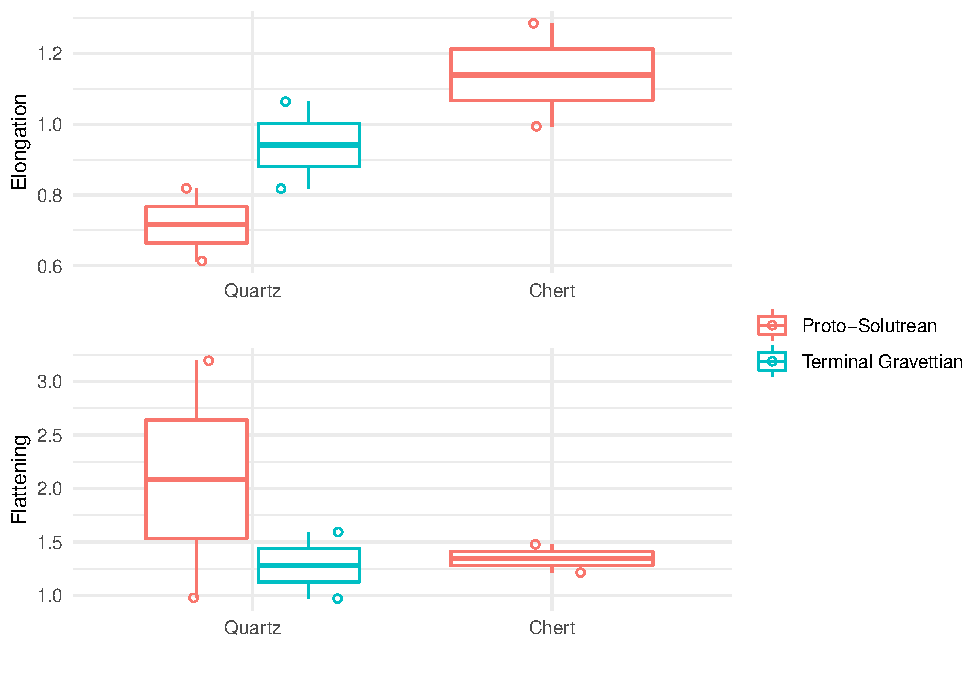
\includegraphics{thesis_files/figure-latex/corebloxplotLP-1.pdf}
\caption{\label{fig:corebloxplotLP}Lapa do Picareiro. Boxplots of core elongation and flattening by raw material and phase.}
\end{figure}
\hypertarget{core-maintenance-products}{%
\subsection{Core maintenance products}\label{core-maintenance-products}}

Core maintenance products are very scarce in the assemblages from both sites, with a single identified piece at Lapa do Picareiro's U/Lower T phase (a chert core tablet), and a total of seven pieces for Vale Boi's assemblages, of which six artifacts come from the Upper 5/4E levels.

At Vale Boi core maintenance products are of two types, core fronts and core tablets (Table \ref{tab:corepreptypeVB}). Most core maintenance products are on chert (n=5) with only two quartz core tablets identified, one for each phase.

No cortex was present in the dorsal surfaces of all core maintenance products. This pattern reveals that maintenance oprations were performed at advanced stages of the reduction sequence.

Finnaly, it is rather interesting the absence of crested pieces from both assemblages, mostly at Vale Boi, where this type of core maintenance product has been referenced for both Solutrean and Gravettian occupations (Cascalheira 2013, Marreiros 2009).
\begin{table}

\caption{\label{tab:corepreptypeVB}Core maintenance products by raw material for Upper 5/4E.}
\centering
\resizebox{\linewidth}{!}{
\begin{tabular}[t]{>{\bfseries}lrrr}
\toprule
Core maintenance product & Chert & Quartz & Total\\
\midrule
CoreFront & 3 & 0 & 3\\
CoreTablet & 2 & 1 & 3\\
Total & 5 & 1 & 6\\
\bottomrule
\end{tabular}}
\end{table}
\hypertarget{flakes}{%
\subsection{Flakes}\label{flakes}}

\hypertarget{vale-boi-5}{%
\subsubsection{Vale Boi}\label{vale-boi-5}}

A total of 1257 flakes were analysed from Vale Boi, 427 of those belonging to Lower 5 group, and 828 to the Upper 5/4E group (Table XXX). This increase was somehow expected according to the abovementioned general intensity of occupation and material density in the transition from one phase to the other. Although there are generally more flakes in quartz, it is obvious the difference in ratios between chert and quartz, when comparing Lower 5 to Upper 5/4E results.
\begin{figure}
\centering
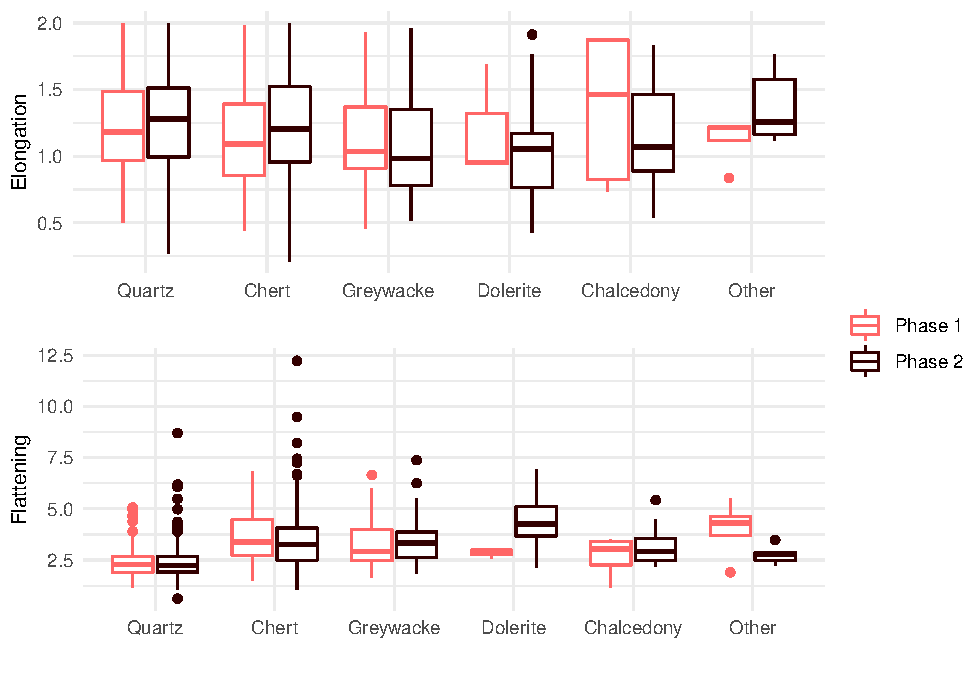
\includegraphics{thesis_files/figure-latex/flakeboxplot-1.pdf}
\caption{\label{fig:flakeboxplot}Vale Boi. Boxplots of flake elongation and flattening by raw material and phase.}
\end{figure}
Morphologically, Lower 5 flakes seem to have mostly irregular shapes, with frequencies over 45\% for most raw materials, followed by convergent and parallel shapes in much lower frequencies (under 15\%) (Table XXX). Dolerite, unlike other raw materials, shows only convergent and parallel shapes even if with low representativity (n=3). Cross sections are mostly irregular and triangular, varying slightly in frequency regarding each raw material, with straight and curved profiles, these two types of profiles representing, each, more than 40\% of chert flakes. All raw materials, with exception of quartz, show high frequencies of straight profiles (over 40\%), chert showing a similar percentage between straight and curved profiles (44.3\% and 42.9\% respectively). Quartz, however, has a frequency of 65\% of straight profiles, showing much smaller frequencies for other types.

On Upper 5/4E, irregular shapes are still frequent, over 25\% on all raw materials, although convergent and parallel shapes show higher frequencies (over 20\%) for quartz, chert and dolerite. Alike Lower 5, cross sections are mostly irregular (over 35\% for most raw materials) or triangular (over 25\% for all raw materials), and profile type show the same patterns and similar percentages as Lower 5.

Unidirectional scar patterns are dominant in both phases and all raw materials, with frequencies over 80\%. Bidirectional patterns are slightly more relevant in chert (9.3\%), and also in dolerite and chalcedony during Upper 5/4E. Dorsal patterns also show a dominance on both phases of 1, 2 and 3 scars for most raw materials, although chert shows the widest numbers and variety for higher scar counts.

Flakes have mostly plain platforms, although for certain raw materials, like quartz, there is a relevant presence of crushed platforms (33.3\% for Lower 5 and 35.9\% for Upper 5/4E). Faceted platforms are present in both phases but in low frequencies, in chert for both Lower 5 (1.4\%) and Upper 5/4E (2.4\%), but in no other raw material. Platforms also mostly non-cortical (between 80\% and 100\% depending on raw material) in both phases.

Blank metrics, including platform measurements, show for Lower 5, the smallest means in chalcedony and dolerite, followed by chert and quartz, where greywacke mean values show bigger Flakes in this raw material. On Upper 5/4E, however, the smallest Flakes are in chert, followed by quartz and chalcedony, where dolerite mean values are fairly closer to those of greywacke, thus making these the Flakes with highest metric mean values.

Regarding elongation, quartz, chert and chalcedony show the highest values, although the latter raw material shows a bigger concentration of similar elongation flakes in the third quartil, thus showing less general elongation. Despite having similar elongation ranges in both groups, quartz shows relatively different medians, on Lower 5 showing a less variability in the lower quartil, while Upper 5/4E shows lower variability in the upper quartil, hinting at a bigger number of consistently elongated quartz flakes in Upper 5/4E. For chert, Upper 5/4E also seems to show higher elongation values for flakes, though once again, there is a wide range of variability within regarding elongation in the assemblage.

As for flattening, quartz shows very low values for flake flattening, compared to other raw materials, although the data also shows the existance of a wide variability within each raw material, with the existance of several outliers which fall from the statistical groupings and quartils. As such, it seems that for all raw materials, perhaps with the exception of quartz, flake flattening is extremely variable in the assemblage.

\hypertarget{lapa-do-picareiro-5}{%
\subsubsection{Lapa do Picareiro}\label{lapa-do-picareiro-5}}

There are a total of plotted 122 Flakes, 46 attributed to the U/Lower T group, more than 50\% being in quartz, and 67 attributed to the Middle T group, its vast majority in chert. On both groups, attributes are very similar.

On the U/Lower T phase, for quartz, there seems to be the predominance of parallel shapes (36.8\%), followed by convergent ones (26.3\%). Chert, however, shows higher percentages for irregular (28.6\%) and divergent (42.9\%) shapes. Cross sections are mostly triangular for all raw materials (over 40\%), although chert also shows high frequencies of trapezoidal cross sections (42.9\%). Profiles are, for all raw materials, mostly straight (57.9\% on quartz and 85.7\% on chert) and terminations show relevant raw material differences, with quartz having bigger frequencies of feathered and hinged terminations (36.8\% both) and chert having a frequency of 42.9\% on pointed terminations. For all raw materials, there is the predominance of unidirectional dorsal patterns, high frequencies over 85\%. Dorsal scars show higher frequencies for 2 and 3 scars on quartz (36.8\% and 42.1\% respectively), while other raw materials show higher frequencies for 3 dorsal scars only (42.9\% on chert).

On the Middle T phase, quartz shows higher frequencies for irregular shapes (53.8\%), followed by convergent ones (38.5\%). Contrary to the patterns seen on the previous group, chert shows higher frequencies for parallel shapes (40.6\%). For all raw materials, cross sections are predominantly triangular (over 40\%) with straight profiles (over 50\%) and feathered terminations for chert (40.6\%), whereas quartz shows higher values for hinged terminations (46.2\%) followed by feathered (38.5\%). Alike the U/Lower T group, there is the predominance of unidirectional dorsal scar patterns (over 90\% for all raw materials), with high frequencies for 2 dorsal scars in quartz (61.5\%) and 2-3 dorsal scars in chert (34.4\% both).

Regarding platforms, for both groups, they are mostly plain for all raw materials (over 40\%), followed by relatively high values of crushed platforms in quartz, with the presence of 1 faceted platform for quartz and chert in each group. Chert on the Middle T group also shows dihedral platforms (18.8\%). Platforms seem to have barely any cortex, for all raw materials in both groups.

Measurements, including platform width and thickness, show larger means for the chert flakes (19.5 mm width and 27.3 mm length), comparatively to the quartz ones (16.7 mm width and 21.8 mm length), for Lower 5 and for Upper 5/4E (chert with 17.2 mm width and 20.9 mm length, and quartz with 13 mm width and 16.3 mm length). There also seems to be a size difference between groups, with the U/Lower T flakes showing bigger means (although with high standard deviation values), while Middle T means show smaller values and smaller SD values, the only constant seeming to be the thickness of flakes on chert (5-5.3 mm), wich seem to show little variability (standard deviations of 3.1 for the U/Lower T group and 2.3 for the Middle T group).
\begin{figure}
\centering
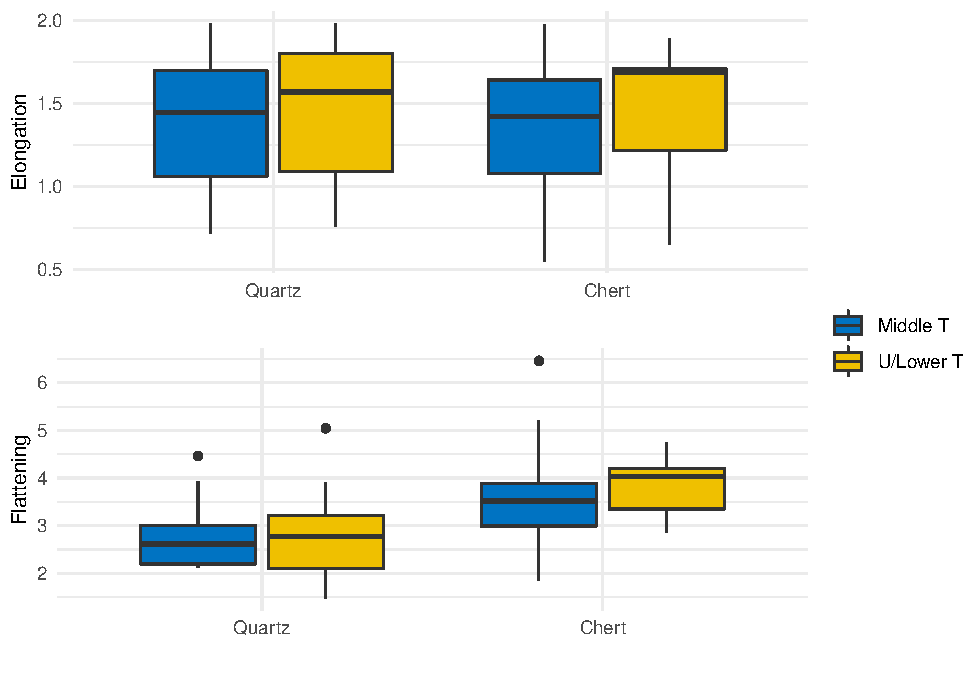
\includegraphics{thesis_files/figure-latex/flakeboxplotLP-1.pdf}
\caption{\label{fig:flakeboxplotLP}Flake elongation and flattening by phase and raw material.}
\end{figure}
Regarding elongation (figure X), values between quartz and chert and even between groups seem to be fairly similar, all with elongation ratios which seem skewed above, thus showing less elongation variability above the 1.5 threshold. Flake flattening, however, shows more apparent differences between raw materials, with quartz showing lower flattening ratios than chert. Within chert, however, there also seems to be a difference in general flattening variability and interquartil skewness, showing a larger number of flakes with similar flattening values (at around 4).

\hypertarget{elongated-blanks}{%
\subsection{Elongated blanks}\label{elongated-blanks}}

\hypertarget{vale-boi-6}{%
\subsubsection{Vale Boi}\label{vale-boi-6}}

There are a total of 219 elongated products in the assemblage (fig X), 82 of them being inserted in Lower 5, while 137 are inserted in Upper 5/4E. Comparatively to blanks, there seems to be a larger number of chert pieces (n=106), this number only changing in Lower 5, where quartz elongated blank numbers (n=44) supersede chert ones (n=31).

For both phases, however, elongated blank attributes are relatively similar, following the same general patterns.

Regarding morphology, elongated blanks have mostly parallel and convergent shapes, on both phases, although Lower 5 shows wider raw material differences, where 63.6\% of quartz has a parallel shapes whereas 51.6\% of chert has convergent ones. Cross sections are mostly triangular, with straight profiles, although there are also high frequencies for curved profiles.

Scar patterns show an obvious tendency for unidirectional knapping strategies on all raw materials. For Lower 5, however, there is the presence of bidirectional scar direction on chert even if in low frequencies (12.9\%), Upper 5/4E showing much lower values for this type of scar pattern, with 2\% on quartz and 4\% on chert. Scar count shows a tendency for 1 to 3 dorsal scars on both phases and all raw materials.

Elongated blanks on both phases seem to be obtained without platform preparation, since most platforms are plain, although quartz also shows crushed platforms. Only two faceted platforms were identified, in Upper 5/4E, on chert and dolerite. The general tendency for both phases is for the nonexistence of cortex on platforms, only certain raw materials showing complete cortical platforms, chert and greywacke on Lower 5 (9.7\% and 16.7\% respectively) and chert on Upper 5/4E (13.3\%).

Finally, elongated products metrics, including platform measurements, show a tendency on both phases for smaller blanks on quartz, followed by chert, where greywacke, dolerite and chalcedony show the biggest blanks and widest platforms. On both stages, means for width, length and thickness for quartz and chert are around 9mm, 21-26mm, 5mm respectively, with higher standard deviation values for length, which is what seems to vary most in these blanks. Despite this, chert elongated blanks seem to show means which hint for higher elongation ratios than quartz.

When plotting width and length for elongated products, by raw material, there seems to be separated groups, for both phases, instead of a continuous dispersion, which may indicate separate production strategies and/or desired dimensions for products.

For Lower 5 there seems to be the existence of one single group for quartz, and two differing groups of width-length combinations for chert (Fig X), although the sample is small, possibly having an impact on the data dispersion. As such, this group in quartz might suggest the preference in Lower 5 for the production of small elongated blanks between 3-10 mm width and under 25 mm length, easily understood by the density curves. This group falls into the definition of bladelet, for the exception of a small quantity of pieces from the latter group, which, due to their width surpassing 12 mm width, are considered blades. Regarding chert, measurements are slightly more dispersed, allowing for the individualization of a wide group of smaller blanks, ranging between 2.5-12 mm width, peaking at around 10 mm, and 10-28 mm length peaking at around 20 mm, again mostly falling into the traditional definition of bladelets. The interpretation of the second group is further truncated by the small sample. The curves show not an increase in density, but instead a maintenance of the curve after a moment of drop, which might not represent a preference. Elongated products in this group have widths and lengths comprehended between 14-17 mm and 30-40 mm respectively, and can be classified as blades.

For Upper 5/4E, quartz continues to have a small sample that seems to show disperse concentrations of products, with a first group of small blanks between 2.5-6 mm width and under 20 mm length, and a second group ranging between 10-12.5 mm width and 20-30 mm length, both classified as bladelets. For quartz, there seems to be a wider dispersion without an obvious peak in the density curve, even within the two groups. For chert, there are three visible concentrations of elongated blanks, although with varying sample numbers on each group: one small group ranging between 2.5-5 mm width and 10-20 mm width, classifying as bladelets; an intermediate group and the best represented in terms of sample numbers, between 8-12.5 mm width and 15-30 mm length, classifying as bladelets with the exception of 2 pieces with slightly exceed the width bladelet limit; a group of larger blanks, with a small sample, ranging between 13-16 mm width and 30-42 mm length, traditionally classified as blades. Regarding the density curves, however, chert seems to peak between 7.5-10 mm width and 20 mm length, showing instead a unimodal curve and possibly, only one prefered width/length ratio with a wider dispersion.
\begin{figure}
\centering
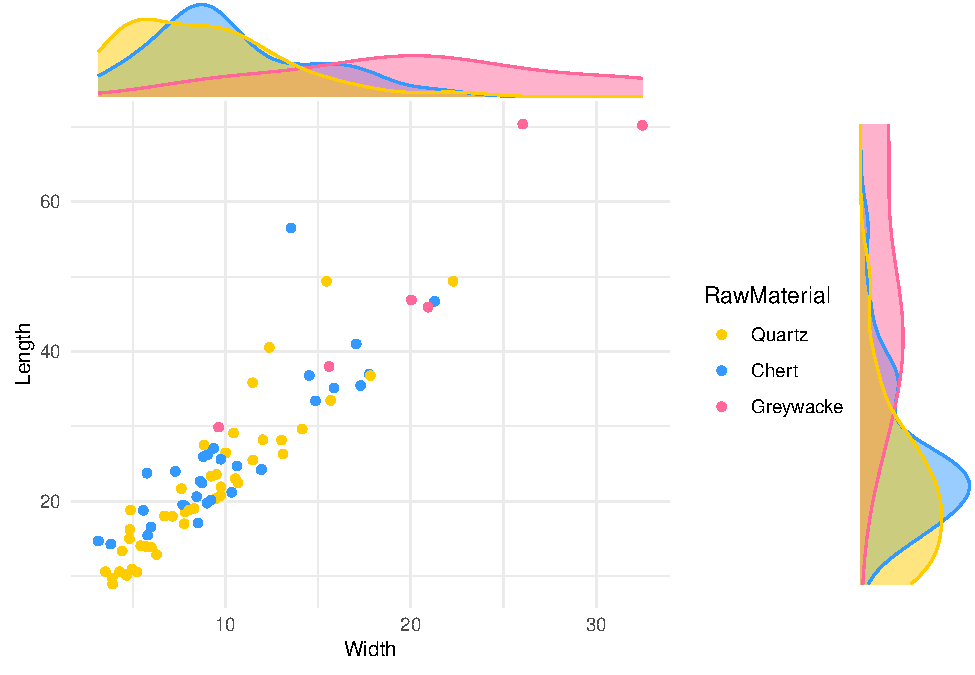
\includegraphics{thesis_files/figure-latex/elongdisp1-1.pdf}
\caption{\label{fig:elongdisp1}Elongated product width and length dispersion by raw material (Lower 5).}
\end{figure}
\begin{figure}
\centering
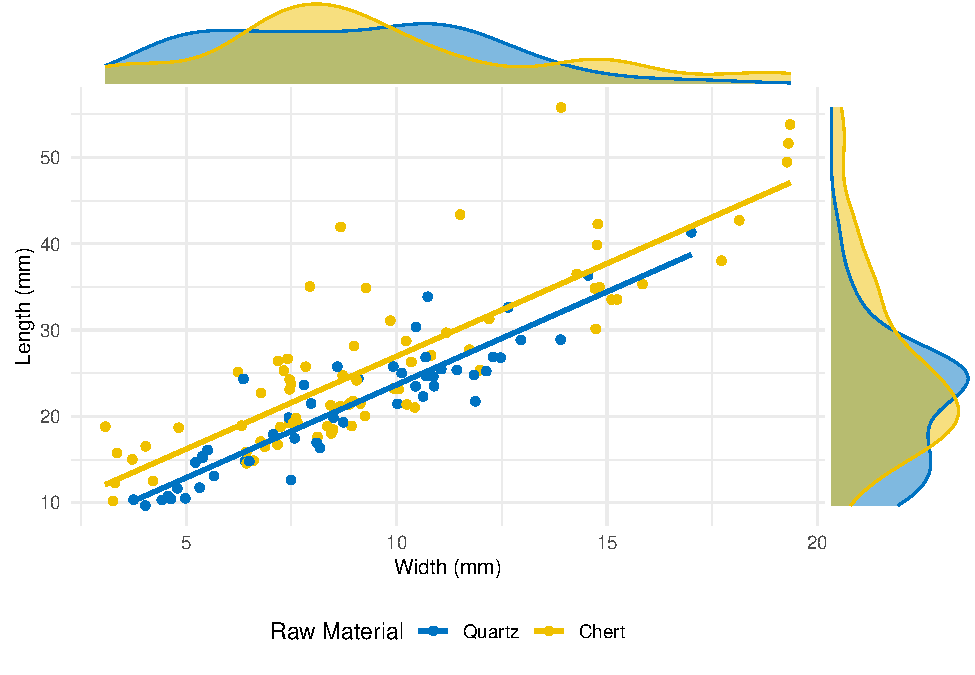
\includegraphics{thesis_files/figure-latex/elongdisp2-1.pdf}
\caption{\label{fig:elongdisp2}Elongated product width and length dispersion by raw material (Upper 5/4E).}
\end{figure}
\hypertarget{lapa-do-picareiro-6}{%
\subsubsection{Lapa do Picareiro}\label{lapa-do-picareiro-6}}

There are a total of plotted 47 elongated blanks, 27 of which belong to the U/Lower T group, more than 50\% on chert, and 20 to the Middle T group, also more than 50\% on chert.

Technological attributes follow closely those already described in blanks, also showing little variation between the U/Lower T and the Middle T.

Elongated blanks show a majority of parallel shapes, followed by convergent, with triangular cross sections, straight profiles followed by curved, with the exception of quartz on the Middle T group, where curved profiles are more frequent. Dorsal scars are unidirectional, with 2 negatives for quartz and 2 to 4 negatives for chert.

Platforms are mostly plain, with no cortex, where quartz seems to have the smaller dimensions.

When plotting width and length for elongated blanks, for chert and quartz, there seems to be two groups of differing dimensions. Regarding the U/Lower T, there is a group of smaller blanks, ranging between 2-10 mm of width and 5-25 mm of length, thus falling into the traditional category of bladelet, and a larger group, although much more disperse and composed mostly of chert, with widths and length ranging between 13-26 mm and 40-60 mm respectively, which may be classified as blades. The density curves for width and length on chert, however, don't seem to show the relevant existance of two groups, with only a continuous increase in values within each variables.

For the Middle T there is also a group of smaller blanks, with width ranging the 3-10 mm width, although length values vary a lot more, going between the 5-30 mm, where the higher values are made up mostly of chert. Even so, this group may be characterized through the traditional classification of bladelet. The second group is made up entirely of chert, although it has less blanks and is very disperse in terms of width, which is higher than 15 mm, and length, higher than 45 mm, also being characterized as blades. Once again, for chert, density curves seem to show a unimodal curve.

These patterns may represent differing production strategies for specific elongated blank sizes and ratios, although, given the altitude of the site, it might simply reflect the truncated reduction sequences present at the site, thus only showing the presence of two wide groups of small elongated blanks and larger elongated blanks. without the intermediate group which wasn't transported into the site.
\begin{figure}
\centering
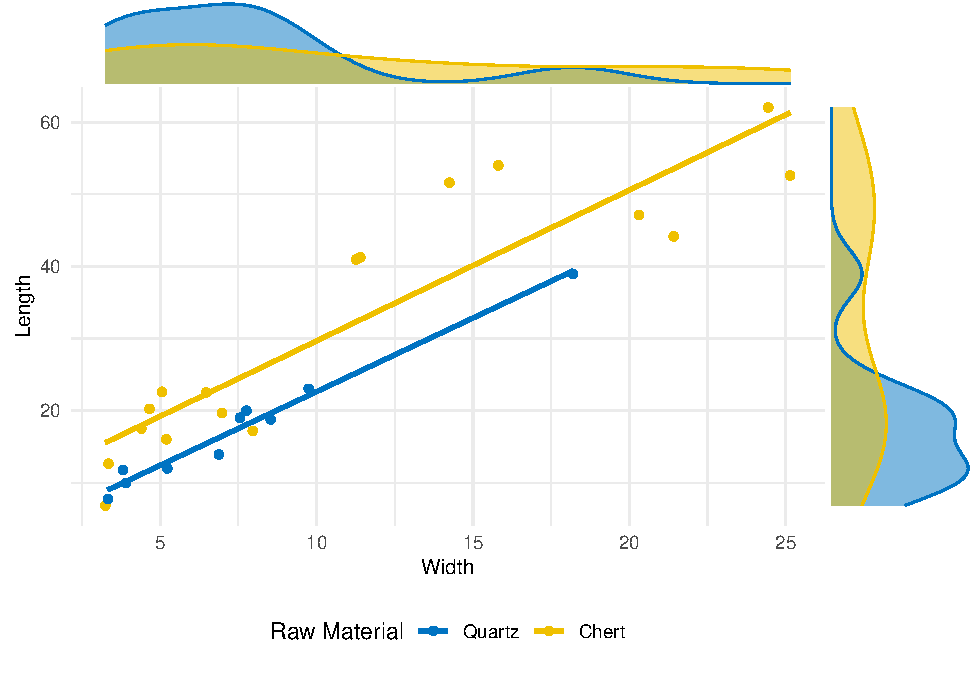
\includegraphics{thesis_files/figure-latex/elongdisp1LP-1.pdf}
\caption{\label{fig:elongdisp1LP}Elongated product width and length dispersion by raw material (U/Lower T).}
\end{figure}
\begin{figure}
\centering
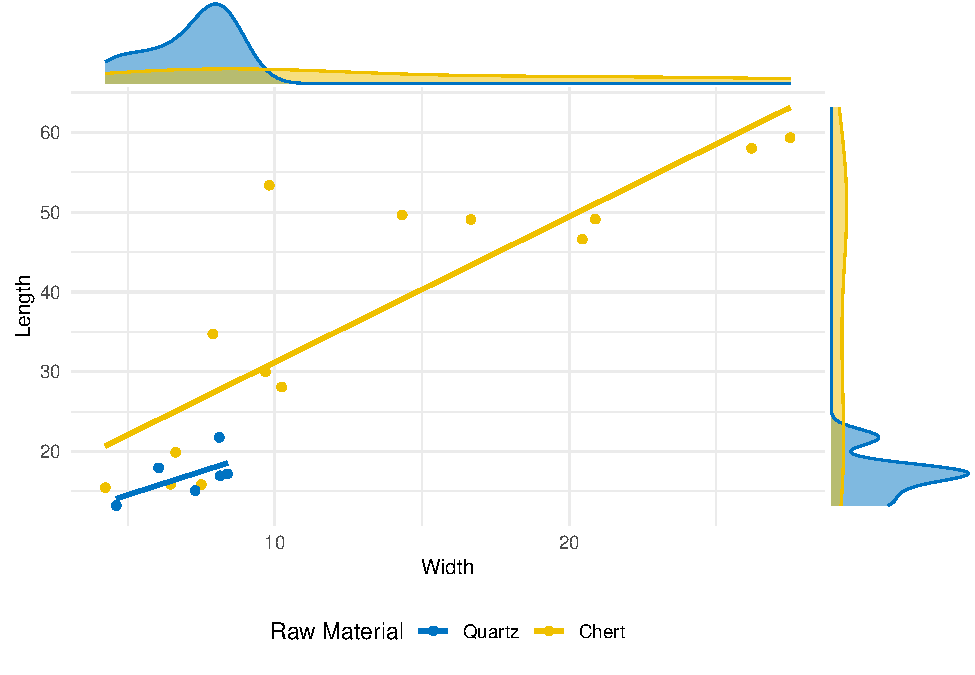
\includegraphics{thesis_files/figure-latex/elongdisp2LP-1.pdf}
\caption{\label{fig:elongdisp2LP}Elongated product width and length dispersion by raw material (Middle T).}
\end{figure}
\hypertarget{retouched-tools}{%
\subsection{Retouched tools}\label{retouched-tools}}

\hypertarget{vale-boi-7}{%
\subsubsection{Vale Boi}\label{vale-boi-7}}

As seen before, retouched pieces make up a small percentage of the assemblage, with 167 identified pieces, from which 55 can be inserted in the Lower 5 group (fig X), while 112 in the Upper 5/4E group (fig X).

Lower 5 is comprised of several typologies, from which a few stand out by their high numbers, such as retouched flakes, corresponding to 27\% of total retouched pieces, mostly in chert, splintered pieces, with 25.4\% of representativity, followed by notches with a frequency of 12.7\%, both occurring in similar numbers in chert (n=6 and n=4 respectively) and quartz (n=8 and n=3).

There is also the presence of endscrapers (9.09\%) and burins (7.27\%), mostly on chert, although their frequencies in the total of retouched pieces is not very representative.

For Upper 5/4E, splintered pieces are still very frequent (24.1\%), in both chert and quartz, followed by endscrapers which represent 22.3\% of the total retouched piece number, most of them in chert, although it may be relevant to point out 2 are made of dolerite. Notches are, once again, the third most frequent retouched typology, with 11.6\% representativity, though most are found in quartz. Every other typology has frequencies under 10\%.

Upper 5/4E thus shows not only a larger number of retouched pieces, which might be the result of a bigger occupation intensity, but also a wider variety of typologies. As Lower 5 shows 11 different retouched piece types, Upper 5/4E shows 16 types, introducing 6 new different typologies, as the double backed blade of stage 1 doesn't appear in the upper occupation.

One of these newly introduced retouched type is the Vale Comprido point, although only representing 5.3\% of retouched piece total for Upper 5/4E. As mentioned before, Vale Comprido points have been identified as a Proto-Solutrean only technological solution, which may appear during the Proto-Solutrean in the Two-phase model, or during either the Terminal Gravettian or Proto-Solutrean in the Three-phase model. Thus, its presence in Upper 5/4E not only conforms to the data already presented for the Portuguese Estremadura (Zilhão 1997) it further strengths the separation of layers 4E and 5 in two moments of differing occupation.

The analysed Vale Comprido points have been identified in chert (n=1), greywacke (n=1), dolerite (n=3) and chalcedony (n=1, which makes up 100\% of retouched pieces made in this raw material). In fact, dolerite had already been identified as a preferred means for making these products (Marreiros 2009), a fact only strengthened by the fact this raw material has more Vale Comprido points than any other, and only appears in one other typology, the endscraper. Comparatively, dolerite doesn't seem to be used for the production of any retouched piece in stage 1. These shall be described into further detail in Chapter 7.4.6.
\begin{landscape}\begin{table}[!h]

\caption{\label{tab:retouchphase1}Lower 5 retouched piece typology by raw material.}
\centering
\resizebox{\linewidth}{!}{
\begin{tabular}[t]{lrlrlrlrlrl}
\toprule
\multicolumn{1}{c}{\textbf{Typology}} & \multicolumn{1}{c}{\textbf{Quartz (n)}} & \multicolumn{1}{c}{\textbf{Quartz (\%)}} & \multicolumn{1}{c}{\textbf{Chert (n)}} & \multicolumn{1}{c}{\textbf{Chert (\%)}} & \multicolumn{1}{c}{\textbf{Greywacke (n)}} & \multicolumn{1}{c}{\textbf{Greywacke (\%)}} & \multicolumn{1}{c}{\textbf{Chalcedony (n)}} & \multicolumn{1}{c}{\textbf{Chalcedony (\%)}} & \multicolumn{1}{c}{\textbf{Total}} & \multicolumn{1}{c}{\textbf{Total (\%)}}\\
\midrule
Endscraper & 0 & 0\% & 4 & 10.53\% & 0 & 0\% & 1 & 100\% & 5 & 9.09\%\\
Dihedral Burin & 1 & 6.67\% & 3 & 7.89\% & 0 & 0\% & 0 & 0\% & 4 & 7.27\%\\
Burin on truncation & 0 & 0\% & 2 & 5.26\% & 0 & 0\% & 0 & 0\% & 2 & 3.64\%\\
Truncation & 0 & 0\% & 1 & 2.63\% & 0 & 0\% & 0 & 0\% & 1 & 1.82\%\\
Notch & 3 & 20\% & 4 & 10.53\% & 0 & 0\% & 0 & 0\% & 7 & 12.73\%\\
\addlinespace
Denticulate & 0 & 0\% & 2 & 5.26\% & 0 & 0\% & 0 & 0\% & 2 & 3.64\%\\
Splintered piece & 8 & 53.33\% & 6 & 15.79\% & 0 & 0\% & 0 & 0\% & 14 & 25.45\%\\
Double backed bladelet & 0 & 0\% & 2 & 5.26\% & 0 & 0\% & 0 & 0\% & 2 & 3.64\%\\
Retouched blade & 0 & 0\% & 1 & 2.63\% & 0 & 0\% & 0 & 0\% & 1 & 1.82\%\\
Retouched bladelet & 0 & 0\% & 2 & 5.26\% & 0 & 0\% & 0 & 0\% & 2 & 3.64\%\\
\addlinespace
Retouched flake & 3 & 20\% & 11 & 28.95\% & 1 & 100\% & 0 & 0\% & 15 & 27.27\%\\
Total & 15 & 100\% & 38 & 100\% & 1 & 100\% & 1 & 100\% & 55 & 100\%\\
\bottomrule
\end{tabular}}
\end{table}
\end{landscape}
\begin{landscape}\begin{table}[!h]

\caption{\label{tab:retouchphase2}Upper 5/4E Retouched piece typology by raw material.}
\centering
\resizebox{\linewidth}{!}{
\begin{tabular}[t]{lrlrlrlrlrlrl}
\toprule
\multicolumn{1}{c}{\textbf{Typology}} & \multicolumn{1}{c}{\textbf{Quartz (n)}} & \multicolumn{1}{c}{\textbf{Quartz (\%)}} & \multicolumn{1}{c}{\textbf{Chert (n)}} & \multicolumn{1}{c}{\textbf{Chert (\%)}} & \multicolumn{1}{c}{\textbf{Greywacke (n)}} & \multicolumn{1}{c}{\textbf{Greywacke (\%)}} & \multicolumn{1}{c}{\textbf{Dolerite (n)}} & \multicolumn{1}{c}{\textbf{Dolerite (\%)}} & \multicolumn{1}{c}{\textbf{Chalcedony (n)}} & \multicolumn{1}{c}{\textbf{Chalcedony (\%)}} & \multicolumn{1}{c}{\textbf{Total}} & \multicolumn{1}{c}{\textbf{Total (\%)}}\\
\midrule
Endscraper & 2 & 5.88\% & 21 & 30\% & 0 & 0\% & 2 & 40\% & 0 & 0\% & 25 & 22.32\%\\
Carinated endscraper & 0 & 0\% & 2 & 2.86\% & 1 & 50\% & 0 & 0\% & 0 & 0\% & 3 & 2.68\%\\
Perforator-endscraper & 0 & 0\% & 1 & 1.43\% & 0 & 0\% & 0 & 0\% & 0 & 0\% & 1 & 0.89\%\\
Perforator & 0 & 0\% & 1 & 1.43\% & 0 & 0\% & 0 & 0\% & 0 & 0\% & 1 & 0.89\%\\
Dihedral Burin & 2 & 5.88\% & 4 & 5.71\% & 0 & 0\% & 0 & 0\% & 0 & 0\% & 6 & 5.36\%\\
\addlinespace
Burin on truncation & 0 & 0\% & 4 & 5.71\% & 0 & 0\% & 0 & 0\% & 0 & 0\% & 4 & 3.57\%\\
Truncation & 0 & 0\% & 4 & 5.71\% & 0 & 0\% & 0 & 0\% & 0 & 0\% & 4 & 3.57\%\\
Notch & 10 & 29.41\% & 3 & 4.29\% & 0 & 0\% & 0 & 0\% & 0 & 0\% & 13 & 11.61\%\\
Denticulate & 1 & 2.94\% & 2 & 2.86\% & 0 & 0\% & 0 & 0\% & 0 & 0\% & 3 & 2.68\%\\
Splintered piece & 15 & 44.12\% & 12 & 17.14\% & 0 & 0\% & 0 & 0\% & 0 & 0\% & 27 & 24.11\%\\
\addlinespace
Backed bladelet & 0 & 0\% & 1 & 1.43\% & 0 & 0\% & 0 & 0\% & 0 & 0\% & 1 & 0.89\%\\
Backed bladelet parcial & 0 & 0\% & 1 & 1.43\% & 0 & 0\% & 0 & 0\% & 0 & 0\% & 1 & 0.89\%\\
Retouched blade & 0 & 0\% & 2 & 2.86\% & 0 & 0\% & 0 & 0\% & 0 & 0\% & 2 & 1.79\%\\
Retouched bladelet & 0 & 0\% & 5 & 7.14\% & 0 & 0\% & 0 & 0\% & 0 & 0\% & 5 & 4.46\%\\
Retouched flake & 4 & 11.76\% & 6 & 8.57\% & 0 & 0\% & 0 & 0\% & 0 & 0\% & 10 & 8.93\%\\
\addlinespace
Total & 34 & 100\% & 70 & 100\% & 2 & 100\% & 5 & 100\% & 1 & 100\% & 112 & 100\%\\
\bottomrule
\end{tabular}}
\end{table}
\end{landscape}
\hypertarget{lapa-do-picareiro-7}{%
\subsubsection{Lapa do Picareiro}\label{lapa-do-picareiro-7}}

The total number of retouched pieces which have spatial information, allowing the identification of phase is 11, of which 6 belong to the U/Lower T group and 5 on the Middle T.

As seen on table X, the U/Lower T shows 4 types of retouched piece typologies, the most present being the retouched flakes (of varied elongation ratios, n=3) all in chert, where the only quartz retouched piece is a splintered piece. From the retouched flakes, one shows similarities with the Vale Comprido point, although the platform/dorsal retouched as to thin the platform is questionable.

For the Middle T group (table x), there is a smaller variety of retouched pieces, all in chert: a notch, retouched flakes (n=2), a truncation and possibly a Vale Comprido point.
\begin{table}[!h]

\caption{\label{tab:retouchTG}U/Lower T retouched piece typology by raw material.}
\centering
\resizebox{\linewidth}{!}{
\begin{tabular}[t]{lrlrlrl}
\toprule
\multicolumn{1}{c}{\textbf{Typology}} & \multicolumn{1}{c}{\textbf{Quartz (n)}} & \multicolumn{1}{c}{\textbf{Quartz (\%)}} & \multicolumn{1}{c}{\textbf{Chert (n)}} & \multicolumn{1}{c}{\textbf{Chert (\%)}} & \multicolumn{1}{c}{\textbf{Total}} & \multicolumn{1}{c}{\textbf{Total (\%)}}\\
\midrule
Dihedral angle burin & 0 & 0\% & 1 & 20\% & 1 & 16.67\%\\
Notch & 0 & 0\% & 1 & 20\% & 1 & 16.67\%\\
Splintered piece & 1 & 100\% & 0 & 0\% & 1 & 16.67\%\\
Retouched flake & 0 & 0\% & 3 & 60\% & 3 & 50\%\\
\bottomrule
\end{tabular}}
\end{table}
\begin{table}[!h]

\caption{\label{tab:retouchPR}Upper 5/4E Retouched piece typology by raw material.}
\centering
\resizebox{\linewidth}{!}{
\begin{tabular}[t]{lrlr}
\toprule
\multicolumn{1}{c}{\textbf{Typology}} & \multicolumn{1}{c}{\textbf{Chert (n)}} & \multicolumn{1}{c}{\textbf{Chert (\%)}} & \multicolumn{1}{c}{\textbf{Total}}\\
\midrule
Concave truncation & 1 & 20\% & 1\\
Vale Comprido point (?) & 1 & 20\% & 1\\
Notch & 1 & 20\% & 1\\
Retouched flake & 2 & 40\% & 2\\
\bottomrule
\end{tabular}}
\end{table}
The analysis of retouched pieces at Lapa do Picareiro is, however, possibly truncated by the edge damage of the assemblage. In all levels, many pieces, both quartz and chert, although in wider quantities in the latter, show variable degrees of edge damage, from light to extensive. Although some edges were obviously damaged by, either trampling or impact by blocks, since there was no homogeneity in its distribution or directionality, some other edges show dubious marks. As such, the present study opted for a more reserved approach regarding the classification of retouch, understanding the caveats of the decision. Thus, retouched pieces, specially the retouched flakes, were only identified as such whenever they displayed homogeneous, localized and unidirectional retouch, which could not be mistaken for edge damage.

\hypertarget{vale-comprido-technology}{%
\subsection{Vale Comprido technology}\label{vale-comprido-technology}}
\begin{figure}
\centering
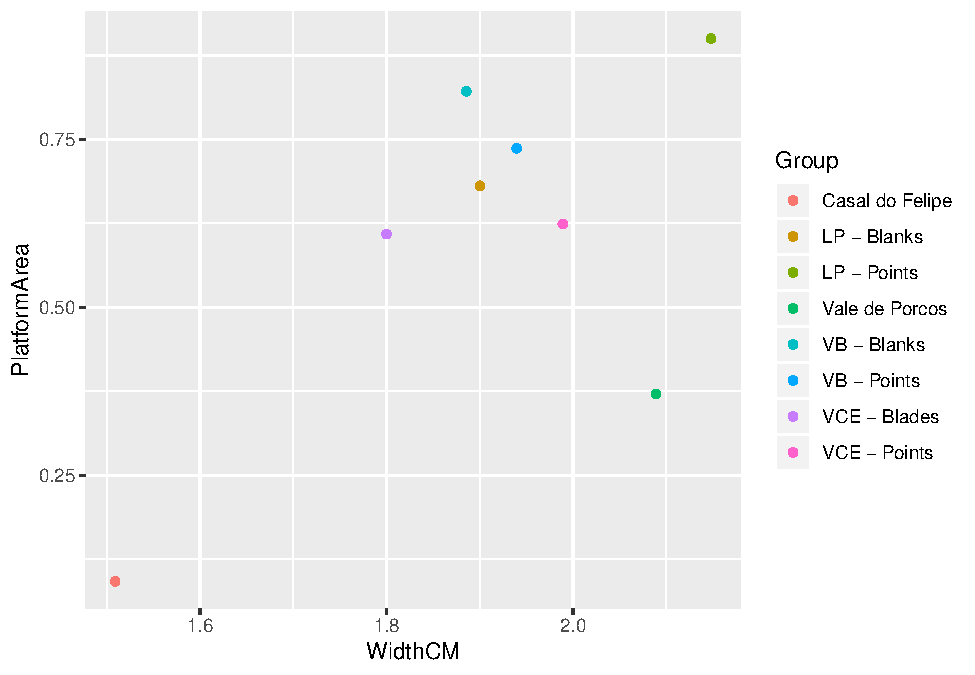
\includegraphics{thesis_files/figure-latex/vca-1.pdf}
\caption{\label{fig:vca}Blank width and platform area of Vale Comprido points and blanks from Vale Boi, Lapa do Picareiro (present analysis) and Casal do Felipe, Vale de Porcos and Vale Comprido - Encosta (Zilhão and Aubry 1995).}
\end{figure}
\begin{figure}
\centering
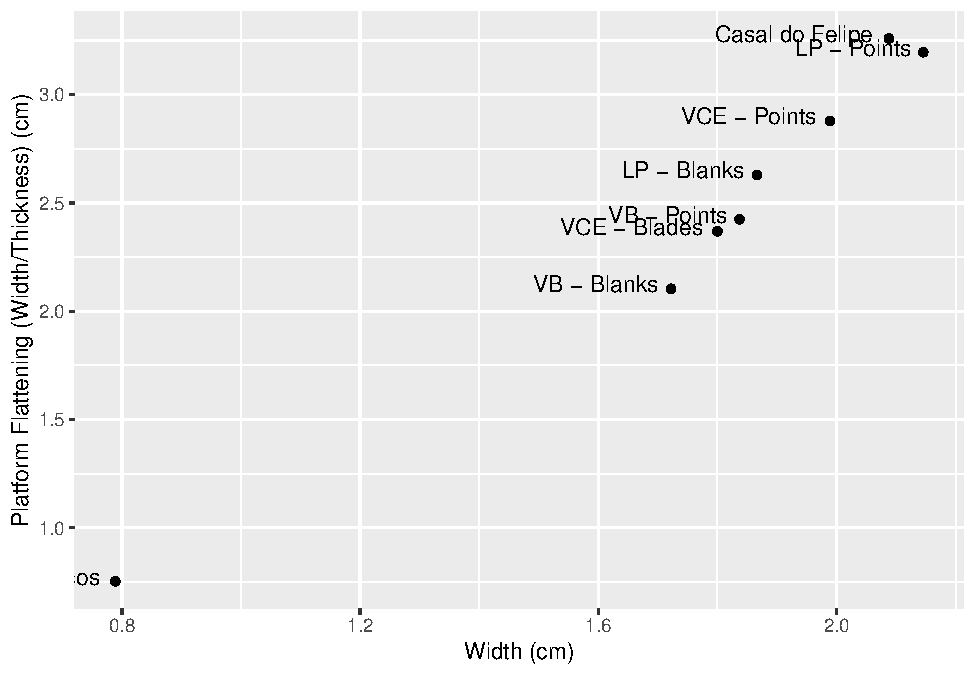
\includegraphics{thesis_files/figure-latex/vcb-1.pdf}
\caption{\label{fig:vcb}Blank width and platform convexity of Vale Comprido points and blanks from Vale Boi, Lapa do Picareiro (present analysis) and Casal do Felipe, Vale de Porcos and Vale Comprido - Encosta (Zilhão and Aubry 1995)}
\end{figure}
\begin{figure}
\centering
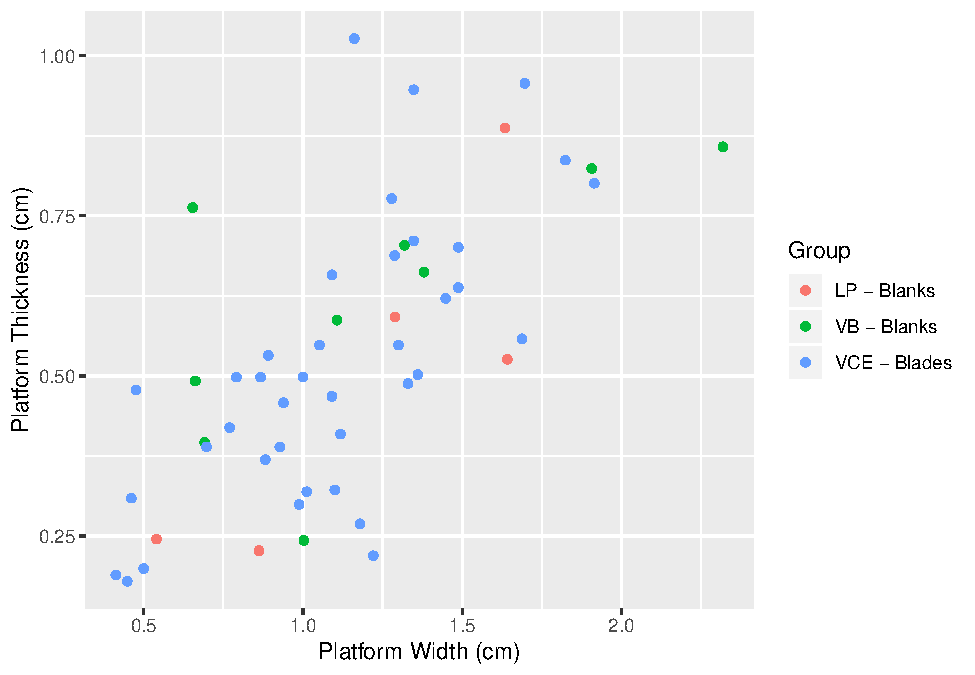
\includegraphics{thesis_files/figure-latex/vcc-1.pdf}
\caption{\label{fig:vcc}Platform width and thickness of Vale Comprido points and blanks from Vale Boi, Lapa do Picareiro (present analysis) and Vale Comprido - Encosta (Zilhão and Aubry 1995).}
\end{figure}
\hypertarget{discussion}{%
\chapter{Discussion}\label{discussion}}

Placeholder

\hypertarget{vale-comprido-technology-1}{%
\section{Vale Comprido technology}\label{vale-comprido-technology-1}}

\hypertarget{conclusion}{%
\chapter*{Conclusion}\label{conclusion}}
\addcontentsline{toc}{chapter}{Conclusion}

If we don't want Conclusion to have a chapter number next to it, we can add the \texttt{\{-\}} attribute.

\textbf{More info}

And here's some other random info: the first paragraph after a chapter title or section head \emph{shouldn't be} indented, because indents are to tell the reader that you're starting a new paragraph. Since that's obvious after a chapter or section title, proper typesetting doesn't add an indent there.

\hypertarget{references}{%
\chapter*{References}\label{references}}
\addcontentsline{toc}{chapter}{References}

\markboth{References}{References}

\noindent

\setlength{\parindent}{-0.20in}
\setlength{\leftskip}{0.20in}
\setlength{\parskip}{8pt}

\hypertarget{appendix}{%
\chapter{Appendix}\label{appendix}}

Placeholder

\hypertarget{refs}{}
\leavevmode\hypertarget{ref-almeida2000}{}%
Almeida, F. (2000). \emph{The terminal gravettian of portuguese estremadura. Technological variability of the lithic industries.} (PhD thesis).

\leavevmode\hypertarget{ref-andrefsky1994}{}%
Andrefsky, W. (1994). Raw-material availability and the organization of technology. \emph{American Antiquity}, \emph{59}(1), 21--34.

\leavevmode\hypertarget{ref-bichoetal2012}{}%
Bicho, N., Cascalheira, J., \& Marreiros, J. (2012). On the (l) edge: The case of vale boi rockshelter (algarve, southern portugal). \emph{Caves in Context. The Economical, Social and Ritual Importance of Caves and Rockshelters}, 65--81.

\leavevmode\hypertarget{ref-cascalheira2010}{}%
Cascalheira, J. (2010). \emph{Tecnologia lítica solutrense do abrigo de vale boi (vila do bispo)}. UNIARQ.

\leavevmode\hypertarget{ref-cascalheira2013}{}%
Cascalheira, J. M. M. (2013). A influência mediterrânica nas redes sociais do solutrense final peninsular.

\leavevmode\hypertarget{ref-inizan1999}{}%
Inizan, M.-L., Reduron-Ballinger, M., Roche, H., \& Tixier, J. (1999). Technology and terminology of knapped stone. \emph{Crep, Nanterre}, 189.

\leavevmode\hypertarget{ref-kempson2011}{}%
Kempson, H., \& Wadley, L. (2011). A review of rock studies for archaeologists, and an analysis of dolerite and hornfels from the sibudu area, KwaZulu-natal. \emph{Southern African Humanities}, \emph{23}(1), 87--107.

\leavevmode\hypertarget{ref-marreiros2009}{}%
Marreiros, J. M. F. (2009). \emph{As primeiras comunidades do homem moderno no algarve ocidental: Caracterização paleotecnológica e paleoetnográfica das comunidades gravetenses e proto-solutrenses de vale boi (algarve, portugal)} (PhD thesis).

\leavevmode\hypertarget{ref-tixier1980}{}%
Tixier, J., \& Inizian, M.-L. (1980). Préhistoire de la pierre taillée. 1. Terminologie et technologie.

\leavevmode\hypertarget{ref-zilhao1997}{}%
Zilhão, J. (1997). \emph{O paleolítico superior da estremadura portuguesa, volume i}.


% Index?

\end{document}
